% Options for packages loaded elsewhere
\PassOptionsToPackage{unicode}{hyperref}
\PassOptionsToPackage{hyphens}{url}
\PassOptionsToPackage{dvipsnames,svgnames,x11names}{xcolor}
%
\documentclass[
  letterpaper,
  DIV=11,
  numbers=noendperiod]{scrreprt}

\usepackage{amsmath,amssymb}
\usepackage{iftex}
\ifPDFTeX
  \usepackage[T1]{fontenc}
  \usepackage[utf8]{inputenc}
  \usepackage{textcomp} % provide euro and other symbols
\else % if luatex or xetex
  \usepackage{unicode-math}
  \defaultfontfeatures{Scale=MatchLowercase}
  \defaultfontfeatures[\rmfamily]{Ligatures=TeX,Scale=1}
\fi
\usepackage{lmodern}
\ifPDFTeX\else  
    % xetex/luatex font selection
\fi
% Use upquote if available, for straight quotes in verbatim environments
\IfFileExists{upquote.sty}{\usepackage{upquote}}{}
\IfFileExists{microtype.sty}{% use microtype if available
  \usepackage[]{microtype}
  \UseMicrotypeSet[protrusion]{basicmath} % disable protrusion for tt fonts
}{}
\makeatletter
\@ifundefined{KOMAClassName}{% if non-KOMA class
  \IfFileExists{parskip.sty}{%
    \usepackage{parskip}
  }{% else
    \setlength{\parindent}{0pt}
    \setlength{\parskip}{6pt plus 2pt minus 1pt}}
}{% if KOMA class
  \KOMAoptions{parskip=half}}
\makeatother
\usepackage{xcolor}
\setlength{\emergencystretch}{3em} % prevent overfull lines
\setcounter{secnumdepth}{5}
% Make \paragraph and \subparagraph free-standing
\ifx\paragraph\undefined\else
  \let\oldparagraph\paragraph
  \renewcommand{\paragraph}[1]{\oldparagraph{#1}\mbox{}}
\fi
\ifx\subparagraph\undefined\else
  \let\oldsubparagraph\subparagraph
  \renewcommand{\subparagraph}[1]{\oldsubparagraph{#1}\mbox{}}
\fi

\usepackage{color}
\usepackage{fancyvrb}
\newcommand{\VerbBar}{|}
\newcommand{\VERB}{\Verb[commandchars=\\\{\}]}
\DefineVerbatimEnvironment{Highlighting}{Verbatim}{commandchars=\\\{\}}
% Add ',fontsize=\small' for more characters per line
\usepackage{framed}
\definecolor{shadecolor}{RGB}{241,243,245}
\newenvironment{Shaded}{\begin{snugshade}}{\end{snugshade}}
\newcommand{\AlertTok}[1]{\textcolor[rgb]{0.68,0.00,0.00}{#1}}
\newcommand{\AnnotationTok}[1]{\textcolor[rgb]{0.37,0.37,0.37}{#1}}
\newcommand{\AttributeTok}[1]{\textcolor[rgb]{0.40,0.45,0.13}{#1}}
\newcommand{\BaseNTok}[1]{\textcolor[rgb]{0.68,0.00,0.00}{#1}}
\newcommand{\BuiltInTok}[1]{\textcolor[rgb]{0.00,0.23,0.31}{#1}}
\newcommand{\CharTok}[1]{\textcolor[rgb]{0.13,0.47,0.30}{#1}}
\newcommand{\CommentTok}[1]{\textcolor[rgb]{0.37,0.37,0.37}{#1}}
\newcommand{\CommentVarTok}[1]{\textcolor[rgb]{0.37,0.37,0.37}{\textit{#1}}}
\newcommand{\ConstantTok}[1]{\textcolor[rgb]{0.56,0.35,0.01}{#1}}
\newcommand{\ControlFlowTok}[1]{\textcolor[rgb]{0.00,0.23,0.31}{#1}}
\newcommand{\DataTypeTok}[1]{\textcolor[rgb]{0.68,0.00,0.00}{#1}}
\newcommand{\DecValTok}[1]{\textcolor[rgb]{0.68,0.00,0.00}{#1}}
\newcommand{\DocumentationTok}[1]{\textcolor[rgb]{0.37,0.37,0.37}{\textit{#1}}}
\newcommand{\ErrorTok}[1]{\textcolor[rgb]{0.68,0.00,0.00}{#1}}
\newcommand{\ExtensionTok}[1]{\textcolor[rgb]{0.00,0.23,0.31}{#1}}
\newcommand{\FloatTok}[1]{\textcolor[rgb]{0.68,0.00,0.00}{#1}}
\newcommand{\FunctionTok}[1]{\textcolor[rgb]{0.28,0.35,0.67}{#1}}
\newcommand{\ImportTok}[1]{\textcolor[rgb]{0.00,0.46,0.62}{#1}}
\newcommand{\InformationTok}[1]{\textcolor[rgb]{0.37,0.37,0.37}{#1}}
\newcommand{\KeywordTok}[1]{\textcolor[rgb]{0.00,0.23,0.31}{#1}}
\newcommand{\NormalTok}[1]{\textcolor[rgb]{0.00,0.23,0.31}{#1}}
\newcommand{\OperatorTok}[1]{\textcolor[rgb]{0.37,0.37,0.37}{#1}}
\newcommand{\OtherTok}[1]{\textcolor[rgb]{0.00,0.23,0.31}{#1}}
\newcommand{\PreprocessorTok}[1]{\textcolor[rgb]{0.68,0.00,0.00}{#1}}
\newcommand{\RegionMarkerTok}[1]{\textcolor[rgb]{0.00,0.23,0.31}{#1}}
\newcommand{\SpecialCharTok}[1]{\textcolor[rgb]{0.37,0.37,0.37}{#1}}
\newcommand{\SpecialStringTok}[1]{\textcolor[rgb]{0.13,0.47,0.30}{#1}}
\newcommand{\StringTok}[1]{\textcolor[rgb]{0.13,0.47,0.30}{#1}}
\newcommand{\VariableTok}[1]{\textcolor[rgb]{0.07,0.07,0.07}{#1}}
\newcommand{\VerbatimStringTok}[1]{\textcolor[rgb]{0.13,0.47,0.30}{#1}}
\newcommand{\WarningTok}[1]{\textcolor[rgb]{0.37,0.37,0.37}{\textit{#1}}}

\providecommand{\tightlist}{%
  \setlength{\itemsep}{0pt}\setlength{\parskip}{0pt}}\usepackage{longtable,booktabs,array}
\usepackage{calc} % for calculating minipage widths
% Correct order of tables after \paragraph or \subparagraph
\usepackage{etoolbox}
\makeatletter
\patchcmd\longtable{\par}{\if@noskipsec\mbox{}\fi\par}{}{}
\makeatother
% Allow footnotes in longtable head/foot
\IfFileExists{footnotehyper.sty}{\usepackage{footnotehyper}}{\usepackage{footnote}}
\makesavenoteenv{longtable}
\usepackage{graphicx}
\makeatletter
\def\maxwidth{\ifdim\Gin@nat@width>\linewidth\linewidth\else\Gin@nat@width\fi}
\def\maxheight{\ifdim\Gin@nat@height>\textheight\textheight\else\Gin@nat@height\fi}
\makeatother
% Scale images if necessary, so that they will not overflow the page
% margins by default, and it is still possible to overwrite the defaults
% using explicit options in \includegraphics[width, height, ...]{}
\setkeys{Gin}{width=\maxwidth,height=\maxheight,keepaspectratio}
% Set default figure placement to htbp
\makeatletter
\def\fps@figure{htbp}
\makeatother
\newlength{\cslhangindent}
\setlength{\cslhangindent}{1.5em}
\newlength{\csllabelwidth}
\setlength{\csllabelwidth}{3em}
\newlength{\cslentryspacingunit} % times entry-spacing
\setlength{\cslentryspacingunit}{\parskip}
\newenvironment{CSLReferences}[2] % #1 hanging-ident, #2 entry spacing
 {% don't indent paragraphs
  \setlength{\parindent}{0pt}
  % turn on hanging indent if param 1 is 1
  \ifodd #1
  \let\oldpar\par
  \def\par{\hangindent=\cslhangindent\oldpar}
  \fi
  % set entry spacing
  \setlength{\parskip}{#2\cslentryspacingunit}
 }%
 {}
\usepackage{calc}
\newcommand{\CSLBlock}[1]{#1\hfill\break}
\newcommand{\CSLLeftMargin}[1]{\parbox[t]{\csllabelwidth}{#1}}
\newcommand{\CSLRightInline}[1]{\parbox[t]{\linewidth - \csllabelwidth}{#1}\break}
\newcommand{\CSLIndent}[1]{\hspace{\cslhangindent}#1}

\KOMAoption{captions}{tableheading}
\makeatletter
\makeatother
\makeatletter
\@ifpackageloaded{bookmark}{}{\usepackage{bookmark}}
\makeatother
\makeatletter
\@ifpackageloaded{caption}{}{\usepackage{caption}}
\AtBeginDocument{%
\ifdefined\contentsname
  \renewcommand*\contentsname{Table of contents}
\else
  \newcommand\contentsname{Table of contents}
\fi
\ifdefined\listfigurename
  \renewcommand*\listfigurename{List of Figures}
\else
  \newcommand\listfigurename{List of Figures}
\fi
\ifdefined\listtablename
  \renewcommand*\listtablename{List of Tables}
\else
  \newcommand\listtablename{List of Tables}
\fi
\ifdefined\figurename
  \renewcommand*\figurename{Figure}
\else
  \newcommand\figurename{Figure}
\fi
\ifdefined\tablename
  \renewcommand*\tablename{Table}
\else
  \newcommand\tablename{Table}
\fi
}
\@ifpackageloaded{float}{}{\usepackage{float}}
\floatstyle{ruled}
\@ifundefined{c@chapter}{\newfloat{codelisting}{h}{lop}}{\newfloat{codelisting}{h}{lop}[chapter]}
\floatname{codelisting}{Listing}
\newcommand*\listoflistings{\listof{codelisting}{List of Listings}}
\makeatother
\makeatletter
\@ifpackageloaded{caption}{}{\usepackage{caption}}
\@ifpackageloaded{subcaption}{}{\usepackage{subcaption}}
\makeatother
\makeatletter
\@ifpackageloaded{tcolorbox}{}{\usepackage[skins,breakable]{tcolorbox}}
\makeatother
\makeatletter
\@ifundefined{shadecolor}{\definecolor{shadecolor}{rgb}{.97, .97, .97}}
\makeatother
\makeatletter
\makeatother
\makeatletter
\makeatother
\ifLuaTeX
  \usepackage{selnolig}  % disable illegal ligatures
\fi
\IfFileExists{bookmark.sty}{\usepackage{bookmark}}{\usepackage{hyperref}}
\IfFileExists{xurl.sty}{\usepackage{xurl}}{} % add URL line breaks if available
\urlstyle{same} % disable monospaced font for URLs
\hypersetup{
  pdftitle={Fundamentos Estadísticos con R},
  pdfauthor={Lic. Juan Isaula},
  colorlinks=true,
  linkcolor={blue},
  filecolor={Maroon},
  citecolor={Blue},
  urlcolor={Blue},
  pdfcreator={LaTeX via pandoc}}

\title{Fundamentos Estadísticos con R}
\author{Lic. Juan Isaula}
\date{Invalid Date}

\begin{document}
\maketitle
\ifdefined\Shaded\renewenvironment{Shaded}{\begin{tcolorbox}[borderline west={3pt}{0pt}{shadecolor}, breakable, frame hidden, enhanced, boxrule=0pt, sharp corners, interior hidden]}{\end{tcolorbox}}\fi

\renewcommand*\contentsname{Table of contents}
{
\hypersetup{linkcolor=}
\setcounter{tocdepth}{2}
\tableofcontents
}
\bookmarksetup{startatroot}

\hypertarget{introducciuxf3n}{%
\chapter*{Introducción}\label{introducciuxf3n}}
\addcontentsline{toc}{chapter}{Introducción}

\markboth{Introducción}{Introducción}

La estadística es el estudio de cómo recopilar, anailizar y sacar
conclusiones de los datos. Es una herramienta enormemente valiosa que se
puede usar para enfocar para e inferir la respuesta a toneladas de
preguntas. Por ejemplo ejemplo, ¿Cuál es la probabilidad de que alguien
compre su producto, cuántas llamadas recibirá su equipo de soporte y
cuántas tallas de jeans debe fabricar para adaptarse al 95\% de la
población? En este curso, usará datos de ventas para descubrir cómo
responder preguntas como estas a medida que que aumenta sus habilidades
estadísticas y aprende a calcular promedios, usar diagramas de
dispersión para mostrar la relación entre valores numéricos y calcular
la correlación. También abordará la probabilidad, la columna vertebral
del razonamiento estadístico, y aprenderá a realizar un estudio bien
deseñado para sacar sus propias conclusiones a partir de los datos.

\bookmarksetup{startatroot}

\hypertarget{summary-resumen-estaduxedstica}{%
\chapter{Summary (resumen)
Estadística}\label{summary-resumen-estaduxedstica}}

Las estadísticas de resumen (summary) le brindan las herramientas que
necesita para reducir conjuntos de datos masivos para revelar los
aspectos más destacados. En este capítulo, explorará estadísticas
resumidas, incluidas la media, mediana y desviación estándar, y
aprenderá a interpretarlas con precisión. También desarrollará sus
habilidades de pensamiento crítico, lo que le permitirá las mejores
estadísticas de resumen para sus datos.

\hypertarget{quuxe9-es-la-estaduxedstica}{%
\section{¿Qué es la estadística ?}\label{quuxe9-es-la-estaduxedstica}}

Es la práctica y el estudio de la recopilación y el análisis de datos.
También podemos hablar de una estadística de resumen, que es un hecho o
un resumen de algunos datos, como un promedio o un conteo.

\hypertarget{quuxe9-pueden-hacer-las-estaduxedsticas}{%
\subsection{¿Qué pueden hacer las
estadísticas?}\label{quuxe9-pueden-hacer-las-estaduxedsticas}}

on el poder de las estadísticas, podemos responder toneladas de
preguntas diferentes como: ¿Qué tan probable es que alguien compre un
producto? ¿Es más probable que las personas lo compren si pueden usar un
sistema de pago diferente? ¿Cuántos ocupantes tendrá su hotel? ¿Cómo se
puede optimizar la ocupación? ¿Cuántas tallas de jeans deben fabricarse
para que le queden al 95\% de la población? ¿Se debe producir el mismo
número de cada tamaño? Una pregunta como, ¿Qué anuncio es más eficaz
para que la gente compre un producto? Se puede responder con pruebas A/B

\hypertarget{quuxe9-no-pueden-hacer-las-estaduxedsticas}{%
\subsection{¿Qué no pueden hacer las
estadísticas?}\label{quuxe9-no-pueden-hacer-las-estaduxedsticas}}

Si bien las estadísticas pueden responder muchas preguntas, es
importante tener en cuenta que las estadísticas no pueden responder
todas las preguntas. Si queremos saber por qué la serie de TV Game of
Thrones es tan popular, podríamos preguntar a todos por qué les gusta,
pero pueden mentir o dejar de lado las razones. Podemos ver si las
series con escenas más violentas atraen a más espectadores, pero incluso
si lo hacen, no podemos saber si la violencia en Game of Throne es la
razón de su popularidad, o si otros factores están impulsando su
popularidad y simplemente sucede.

\hypertarget{tipos-de-estaduxedsticas}{%
\subsection{Tipos de Estadísticas}\label{tipos-de-estaduxedsticas}}

Hay dos ramas principales de la estadística:

\begin{itemize}
\item
  Estadística Descriptiva
\item
  Estadística Inferencial
\end{itemize}

\hypertarget{estaduxedstica-descriptiva}{%
\subsubsection{Estadística
Descriptiva}\label{estaduxedstica-descriptiva}}

Este tipo de estadística se centra en describir y resumir los datos
disponibles. Después de preguntar a cuatro amigos cómo llegan al
trabajo, podemos ver que el 50\% de ellos conducen al trabajo, el 25\%
van en autobús y el 25\% en bicicleta. Estos son ejemplos de
estadísticas descriptivas.

\hypertarget{estaduxedstica-inferencial}{%
\subsubsection{Estadística
Inferencial}\label{estaduxedstica-inferencial}}

Este tipo de estadística utiliza los datos disponibles, que se denominan
datos de muestra, para hacer inferencia sobre una población más grande.
Podríamos usar estadísticas inferenciasles para determinar que
porcentaje de personas conducen al trabajo en función de nuestros datos
de muestra.

\hypertarget{tipos-de-datos}{%
\subsection{Tipos de Datos}\label{tipos-de-datos}}

Existen dos tipos principales de datos. Los datos númericos o
cuantitativos se componen de valores numéricos. Los datos categóricos o
cualitativos están formados por valores que pertenecen a distintos
grupos. Es importante tener en cuenta que estos no son los únicos tipos
de datos que existen; también hay otros, pero nos centraremos en estos
dos. Los datos numéricos se pueden separar en datos:

\begin{itemize}
\item
  continuos, y
\item
  discretos.
\end{itemize}

Los datos \texttt{numéricos\ continuos} suelen ser cantidades que pueden
medir, como la velocidad o el tiempo. Los datos
\texttt{numéricos\ discretos} suelen ser datos de conteo, como la
cantidad de mascotas o la cantidad de paquetes enviados. Los datos
categóricos pueden ser nominales o ordinales.

\begin{itemize}
\item
  Los datos categóricos nominales se componen de categorías sin orden
  inherente, como el estado civil o el país de residencia.
\item
  Los datos categóricos ordinales tienen un orden inherente, como una
  una pregunta de encuesta donde debe indicar el grado en que está de
  acuerdo con una afirmación.
\end{itemize}

\hypertarget{los-datos-categuxf3ricos-se-pueden-presentar-como-nuxfameros}{%
\subsection{Los datos categóricos se pueden presentar como
números}\label{los-datos-categuxf3ricos-se-pueden-presentar-como-nuxfameros}}

A veces, las variables categóricas se representan mediante números. Los
casados y solteros se pueden representar usando 1 y 0, o una escala del
1 al 5. Sin embargo es importante tener en cuenta que esto no
necesariamente los convierte en variables númericas.

\hypertarget{por-quuxe9-es-importante-el-tipo-de-dato}{%
\subsection{¿Por qué es importante el tipo de
dato?}\label{por-quuxe9-es-importante-el-tipo-de-dato}}

Ser capaz de identificar los tipos de datos es importante, ya que el
tipo de datos con los que está trabajando dictará qué tipos de
estadística de resumen y visualizaciones tienen sentido para sus datos,
por lo que esta es una habilidad importante que debe dominar. Para datos
numericós, podemos usar estadísticas de resumen como la media y gráficos
como diagramas de dispersión, pero estos no tienen mucho sentido para
los datos categóricos.

Veamos el siguiente ejemplo, para comenzar a diferenciar la estadística
descriptiva de la inferencial

\begin{longtable}[]{@{}
  >{\raggedright\arraybackslash}p{(\columnwidth - 2\tabcolsep) * \real{0.5417}}
  >{\raggedright\arraybackslash}p{(\columnwidth - 2\tabcolsep) * \real{0.4583}}@{}}
\toprule\noalign{}
\begin{minipage}[b]{\linewidth}\raggedright
Descriptiva
\end{minipage} & \begin{minipage}[b]{\linewidth}\raggedright
Inferencial
\end{minipage} \\
\midrule\noalign{}
\endhead
\bottomrule\noalign{}
\endlastfoot
Teniendo en cuenta los datos de cada solicitud de sevicio al cliente
realizada, ¿Cuál es el tiempo promedio que se tardo en responder? &
Después de entrevistar a 100 clientes, ¿Qué porcentaje de todos sus
clientes está satisfecho con su producto? \\
Dados los datos de las 100,000 personas que vieron el anuncio ¿Qué
porcentaje de personas hizo click en el? & Dados los datos de 20 peces
capturados en un lago, ¿cuál es el peso promedio de todos los peces del
lago? \\
\end{longtable}

Ahora, hagamos un ejercicio similar para identificar el tipo de dato.

\begin{longtable}[]{@{}
  >{\raggedright\arraybackslash}p{(\columnwidth - 4\tabcolsep) * \real{0.3562}}
  >{\raggedright\arraybackslash}p{(\columnwidth - 4\tabcolsep) * \real{0.3836}}
  >{\raggedright\arraybackslash}p{(\columnwidth - 4\tabcolsep) * \real{0.2603}}@{}}
\toprule\noalign{}
\begin{minipage}[b]{\linewidth}\raggedright
numérico (continuo)
\end{minipage} & \begin{minipage}[b]{\linewidth}\raggedright
numérico (discreto)
\end{minipage} & \begin{minipage}[b]{\linewidth}\raggedright
categórico
\end{minipage} \\
\midrule\noalign{}
\endhead
\bottomrule\noalign{}
\endlastfoot
Kilovatios de electricidad utilizados & Número de cursos de estadística
tomados & Marca de un producto \\
Temperatura del aire & Número de artículos en Stock & Código Postal \\
& Número de click en un anuncio & \\
\end{longtable}

\hypertarget{medidas-del-centro}{%
\section{Medidas del Centro}\label{medidas-del-centro}}

En esta sección, comenzaremos a analizar las estadísticas de resumen,
algunas de las cuales quizás ya le resulten familiares, como la
\texttt{media} y la \texttt{mediana}.

\hypertarget{datos-de-sueuxf1o-de-mamiferos}{%
\subsection{Datos de sueño de
mamiferos}\label{datos-de-sueuxf1o-de-mamiferos}}

Veremos los datos sobre los hábitos de sueño de diferentes mamíferos.
Estos datos ya estan precargados por defecto en \texttt{R} en el paquete
o librería de \texttt{ggplot2}, veamos como acceder a ellos en R.

\begin{Shaded}
\begin{Highlighting}[]
\FunctionTok{library}\NormalTok{(ggplot2)  }
\FunctionTok{data}\NormalTok{(}\StringTok{"msleep"}\NormalTok{) }
\NormalTok{msleep}
\end{Highlighting}
\end{Shaded}

\begin{verbatim}
# A tibble: 83 x 11
   name   genus vore  order conservation sleep_total sleep_rem sleep_cycle awake
   <chr>  <chr> <chr> <chr> <chr>              <dbl>     <dbl>       <dbl> <dbl>
 1 Cheet~ Acin~ carni Carn~ lc                  12.1      NA        NA      11.9
 2 Owl m~ Aotus omni  Prim~ <NA>                17         1.8      NA       7  
 3 Mount~ Aplo~ herbi Rode~ nt                  14.4       2.4      NA       9.6
 4 Great~ Blar~ omni  Sori~ lc                  14.9       2.3       0.133   9.1
 5 Cow    Bos   herbi Arti~ domesticated         4         0.7       0.667  20  
 6 Three~ Brad~ herbi Pilo~ <NA>                14.4       2.2       0.767   9.6
 7 North~ Call~ carni Carn~ vu                   8.7       1.4       0.383  15.3
 8 Vespe~ Calo~ <NA>  Rode~ <NA>                 7        NA        NA      17  
 9 Dog    Canis carni Carn~ domesticated        10.1       2.9       0.333  13.9
10 Roe d~ Capr~ herbi Arti~ lc                   3        NA        NA      21  
# i 73 more rows
# i 2 more variables: brainwt <dbl>, bodywt <dbl>
\end{verbatim}

Antes de sumerginos en esto, recordemos cómo funcionan los histogramas.
Un histograma toma un montón de puntos de datos y los separa en
contenedores o rangos de valores.

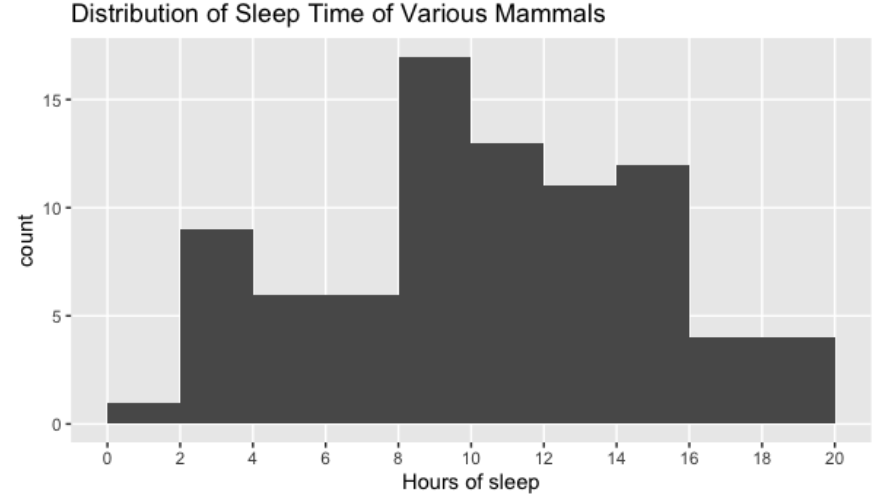
\includegraphics{fig2.png}

Aquí hay un contenedor de 0 a 2 horas, de 2 a 4 horas y así
sucesivamente. Las alturas de las barras representan las cantidad de
puntos de datos que caen en ese contenedor, por lo que hay un mamífero
en el conjunto de datos que duerme entre 0 y 2 horas, y nueve mamíferos
que duermen de dos a cuatro horas. Los histogramas son una excelente
manera de resumir visualmente los datos, pero podemos usar estadísticas
de resumen numérico para resumir aún más.

\hypertarget{cuuxe1nto-tiempo-suelen-dormir-los-mamuxedferos-de-este-conjunto-de-datos}{%
\subsection{¿Cuánto tiempo suelen dormir los mamíferos de este conjunto
de datos
?}\label{cuuxe1nto-tiempo-suelen-dormir-los-mamuxedferos-de-este-conjunto-de-datos}}

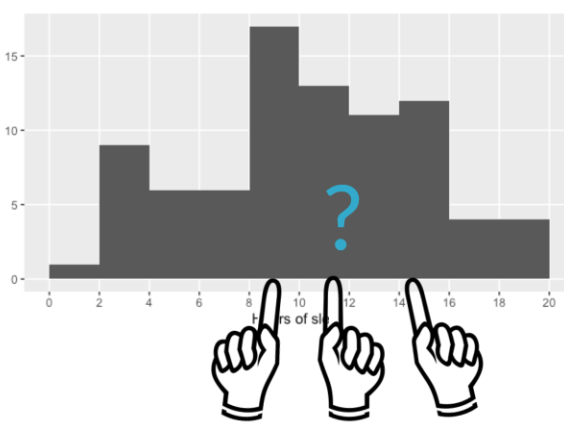
\includegraphics{fig3.png}

Una forma de resumir los datos es respondiendo a la pregunta de esta
sección. Para responder a esto, necesitamos averiguar cuál es el valor
\texttt{típico} o \texttt{central} de los datos. Discutiremos tres
definiciones diferentes, o medidas de centro:

\begin{enumerate}
\def\labelenumi{\arabic{enumi}.}
\tightlist
\item
  Media
\item
  Mediana
\item
  Moda
\end{enumerate}

\hypertarget{medidas-del-centro-1}{%
\section{Medidas del Centro}\label{medidas-del-centro-1}}

\hypertarget{media}{%
\subsection{Media}\label{media}}

La media, a menudo llamada promedio, es una de las formas más comunes de
resumir los datos. Para calcular la media, sumamos todos los números de
interés y los dividimos por el número total de puntos de datos, que aquí
es 83.

\[
media = \bar{x} = \frac{1}{n}\sum_{i=1}^n x_i
\]

Esto nos da 10 punto 43 horas de sueño. En \texttt{R}, podemos usar la
función \texttt{mean()} pasándole la variable de interés.

\begin{Shaded}
\begin{Highlighting}[]
\FunctionTok{mean}\NormalTok{(msleep}\SpecialCharTok{$}\NormalTok{sleep\_total)}
\end{Highlighting}
\end{Shaded}

\begin{verbatim}
[1] 10.43373
\end{verbatim}

\hypertarget{mediana}{%
\subsection{Mediana}\label{mediana}}

Otra medida de centro es la mediana. La mediana es el valor en el que el
50\% de los datos es inferior y el 50\% de los datos es superior.
Podemos calcular esto ordenando todos los puntos de datos y tomando el
del medio, que sería el indice 42 en este caso.

\begin{Shaded}
\begin{Highlighting}[]
\FunctionTok{sort}\NormalTok{(msleep}\SpecialCharTok{$}\NormalTok{sleep\_total)}
\end{Highlighting}
\end{Shaded}

\begin{verbatim}
 [1]  1.9  2.7  2.9  3.0  3.1  3.3  3.5  3.8  3.9  4.0  4.4  5.2  5.3  5.3  5.4
[16]  5.6  6.2  6.3  6.3  7.0  7.7  8.0  8.3  8.4  8.4  8.6  8.7  8.7  8.9  9.1
[31]  9.1  9.4  9.4  9.5  9.6  9.7  9.8  9.8 10.0 10.1 10.1 10.1 10.3 10.3 10.4
[46] 10.6 10.9 11.0 11.0 11.1 11.3 11.5 12.1 12.5 12.5 12.5 12.5 12.8 12.8 13.0
[61] 13.5 13.7 13.8 14.2 14.3 14.4 14.4 14.5 14.6 14.9 14.9 15.6 15.8 15.8 15.9
[76] 16.6 17.0 17.4 18.0 18.1 19.4 19.7 19.9
\end{verbatim}

Esto nos da una mediana de 10.1 horas de sueño.

\begin{Shaded}
\begin{Highlighting}[]
\FunctionTok{sort}\NormalTok{(msleep}\SpecialCharTok{$}\NormalTok{sleep\_total)[}\DecValTok{42}\NormalTok{]}
\end{Highlighting}
\end{Shaded}

\begin{verbatim}
[1] 10.1
\end{verbatim}

En R, podemos usar la función \texttt{median()} para hacer los cálculos
por nosotros.

\begin{Shaded}
\begin{Highlighting}[]
\FunctionTok{median}\NormalTok{(msleep}\SpecialCharTok{$}\NormalTok{sleep\_total)}
\end{Highlighting}
\end{Shaded}

\begin{verbatim}
[1] 10.1
\end{verbatim}

\hypertarget{la-moda}{%
\subsection{La Moda}\label{la-moda}}

La moda es el valor más frecuente en los datos. Si contamos cuantas
ocurrencias hay dentro de cada \texttt{sleep\_total} y ordenamos en
orden descendente, veamos

\begin{Shaded}
\begin{Highlighting}[]
\FunctionTok{library}\NormalTok{(tidyverse)}
\end{Highlighting}
\end{Shaded}

\begin{verbatim}
-- Attaching core tidyverse packages ------------------------ tidyverse 2.0.0 --
v dplyr     1.1.2     v readr     2.1.4
v forcats   1.0.0     v stringr   1.5.0
v lubridate 1.9.2     v tibble    3.2.1
v purrr     1.0.1     v tidyr     1.3.0
-- Conflicts ------------------------------------------ tidyverse_conflicts() --
x dplyr::filter() masks stats::filter()
x dplyr::lag()    masks stats::lag()
i Use the conflicted package (<http://conflicted.r-lib.org/>) to force all conflicts to become errors
\end{verbatim}

\begin{Shaded}
\begin{Highlighting}[]
\NormalTok{msleep }\SpecialCharTok{\%\textgreater{}\%} \FunctionTok{count}\NormalTok{(sleep\_total, }\AttributeTok{sort =} \ConstantTok{TRUE}\NormalTok{)}
\end{Highlighting}
\end{Shaded}

\begin{verbatim}
# A tibble: 65 x 2
   sleep_total     n
         <dbl> <int>
 1        12.5     4
 2        10.1     3
 3         5.3     2
 4         6.3     2
 5         8.4     2
 6         8.7     2
 7         9.1     2
 8         9.4     2
 9         9.8     2
10        10.3     2
# i 55 more rows
\end{verbatim}

note que hay 4 mamiferos que duermen durante 12.5 horas, así que esta es
la moda. La moda de la variable \texttt{vore} del conjunto de datos, que
indica la dieta del animal es herbívora, veamomos:

\begin{Shaded}
\begin{Highlighting}[]
\NormalTok{msleep }\SpecialCharTok{\%\textgreater{}\%} \FunctionTok{count}\NormalTok{(vore, }\AttributeTok{sort =} \ConstantTok{TRUE}\NormalTok{)}
\end{Highlighting}
\end{Shaded}

\begin{verbatim}
# A tibble: 5 x 2
  vore        n
  <chr>   <int>
1 herbi      32
2 omni       20
3 carni      19
4 <NA>        7
5 insecti     5
\end{verbatim}

La moda se usa a menudo para variables categóricas, ya que las variables
categóricas, pueden estar desordenadas y, a menudo no tienen una
representación numérica inherente.

\hypertarget{agregar-un-valor-atuxedpico}{%
\section{Agregar un valor atípico}\label{agregar-un-valor-atuxedpico}}

Ahora que tenemos muchas formas de medir el centro, ¿cómo sabemos cuál
usar? Veamos un ejemplo. Aquí, tenemos todos los insectivoros en el
conjunto de datos

\begin{Shaded}
\begin{Highlighting}[]
\NormalTok{msleep }\SpecialCharTok{\%\textgreater{}\%} 
  \FunctionTok{filter}\NormalTok{(vore }\SpecialCharTok{==} \StringTok{"insecti"}\NormalTok{) }\SpecialCharTok{\%\textgreater{}\%} 
  \FunctionTok{summarize}\NormalTok{(}\AttributeTok{mean\_sleep =} \FunctionTok{mean}\NormalTok{(sleep\_total),}
            \AttributeTok{median\_sleep =} \FunctionTok{median}\NormalTok{(sleep\_total))}
\end{Highlighting}
\end{Shaded}

\begin{verbatim}
# A tibble: 1 x 2
  mean_sleep median_sleep
       <dbl>        <dbl>
1       14.9         18.1
\end{verbatim}

Obtenemos un tiempo de sueño medio de 14.94 horas y un tiempo de sueño
medio de 18.1 horas.

Ahora digamos que hemos descubierto un nuevo insectívoro misterioso que
nunca duerme.

Si volvemos a tomar la media y mediana, obtenemos resultados diferentes.
La media se puede reducir en más de 3 horas, mientras que la mediana
cambió en menos de una hora. Esto se debe a que la media es mucho más
sensible a los valores extremos que la mediana.

Dado que la media es más sensible a los valores extremos, funciona mejor
para datos simétricos como este.

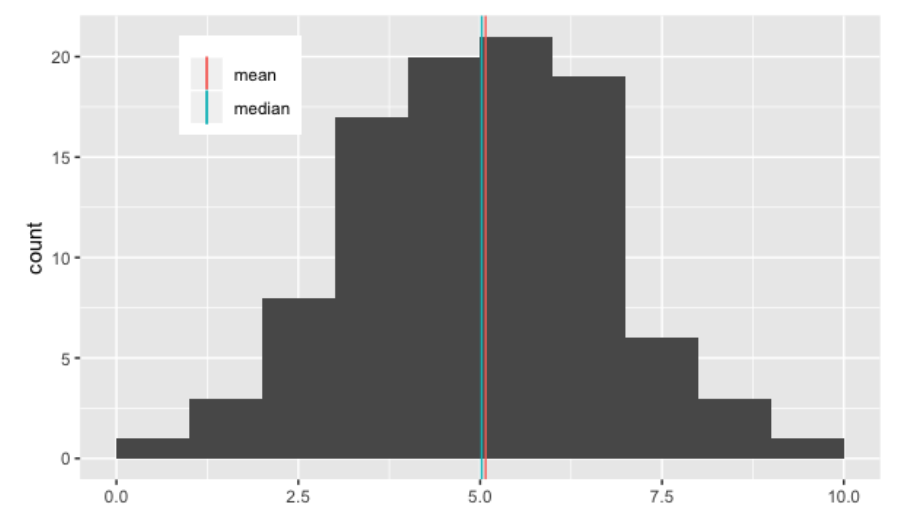
\includegraphics{fig4.png}

Observe que la media, en rojo, y la mediana en verde, estan bastante
cerca.

\hypertarget{sesgo}{%
\section{Sesgo}\label{sesgo}}

Sin embargo, si los datos estan sesgados, lo que significa que no son
simétricos, como se muestra en la figura siguiente

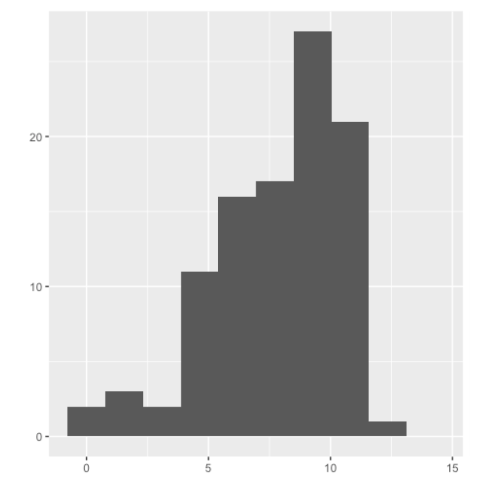
\includegraphics{fig5.png}

generalmente es mejor usar la mediana. En este histograma, note que los
datos se apilan a la derecha. Los datos que se ven así se denominan
datos asimétricos a la izquierda. Cuando los datos se acumulan a la
izquierda, están sesgados a la derecha, vea la siguiente figura.

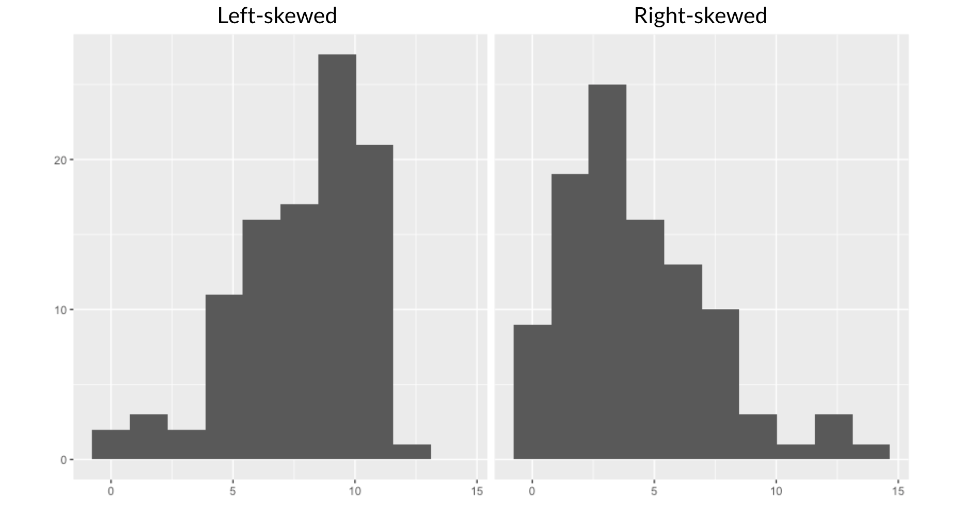
\includegraphics{fig6.png}

Cuando los datos están sesgados, la media y la mediana son diferentes.
La media se tira en dirección del sesgo, por lo que es más baja que la
mediana en los datos sesgados a la izquierda y más alta que la mediana
en los datos sesgados a la derecha.

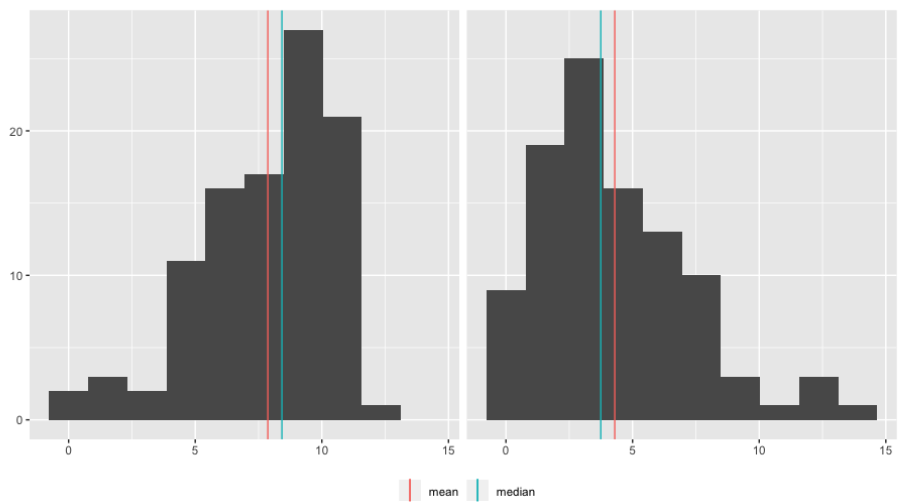
\includegraphics{fig7.png}

Debido a que la media se ve afectada por los valores extremos, es mejor
usar la mediana, ya que se ve menos afectada por los valores atípicos.

\hypertarget{ejercicio-1}{%
\section{Ejercicio 1}\label{ejercicio-1}}

En este capítulo, trabajaremos con el indice de huella de carbono
alimentario 2018. El conjunto de datos \texttt{food\_consumption}
contiene información sobre los kilogramos de alimentos consumidos por
persona por año en cada país en cada categoría de alimentos
(\texttt{consumption)}, así como información sobre la huella de carbono
de esa categoría de alimentos (\texttt{co2\_emissions}) medida en
kilogramos de dióxido de carbono o \(CO_2\), por persona por año en cada
país.

En este ejercicio, nos encargaremos de calcular medidas de centro para
comparar el consumo de alimentos en EE.UU y Bélgica.

\begin{itemize}
\tightlist
\item
  Primero creamos dos marcos de datos: uno que contenga las filas de
  \texttt{food\_consumption} para \texttt{Bélgica} y otro que contenga
  las filas de \texttt{USA}. Llamaremos a estos marcos de datos como
  \texttt{belgica\_consumption} y \texttt{usa\_consumption}. Veamos como
  hacerlo en R.
\end{itemize}

\begin{Shaded}
\begin{Highlighting}[]
\CommentTok{\# Primero cargamos el conjunto de datos}
\NormalTok{food\_consumption }\OtherTok{\textless{}{-}} \FunctionTok{readRDS}\NormalTok{(}\StringTok{"food\_consumption.rds"}\NormalTok{)}

\NormalTok{belgica\_consumption }\OtherTok{\textless{}{-}}\NormalTok{ food\_consumption }\SpecialCharTok{\%\textgreater{}\%} 
  \FunctionTok{filter}\NormalTok{(country }\SpecialCharTok{==} \StringTok{"Belgium"}\NormalTok{)}

\NormalTok{usa\_consumption }\OtherTok{\textless{}{-}}\NormalTok{ food\_consumption }\SpecialCharTok{\%\textgreater{}\%} 
  \FunctionTok{filter}\NormalTok{(country }\SpecialCharTok{==} \StringTok{"USA"}\NormalTok{)}
\end{Highlighting}
\end{Shaded}

Ahora, calculamos la media y mediana de kilogramos de alimentos
consumidos por persona por año para ambos países.

\begin{itemize}
\tightlist
\item
  \textbf{\emph{Bélgica}}
\end{itemize}

\begin{Shaded}
\begin{Highlighting}[]
\FunctionTok{mean}\NormalTok{(belgica\_consumption}\SpecialCharTok{$}\NormalTok{consumption)}
\end{Highlighting}
\end{Shaded}

\begin{verbatim}
[1] 42.13273
\end{verbatim}

\begin{Shaded}
\begin{Highlighting}[]
\FunctionTok{median}\NormalTok{(belgica\_consumption}\SpecialCharTok{$}\NormalTok{consumption)}
\end{Highlighting}
\end{Shaded}

\begin{verbatim}
[1] 12.59
\end{verbatim}

\begin{itemize}
\tightlist
\item
  \textbf{\emph{Usa}}
\end{itemize}

\begin{Shaded}
\begin{Highlighting}[]
\FunctionTok{mean}\NormalTok{(usa\_consumption}\SpecialCharTok{$}\NormalTok{consumption)}
\end{Highlighting}
\end{Shaded}

\begin{verbatim}
[1] 44.65
\end{verbatim}

\begin{Shaded}
\begin{Highlighting}[]
\FunctionTok{median}\NormalTok{(usa\_consumption}\SpecialCharTok{$}\NormalTok{consumption)}
\end{Highlighting}
\end{Shaded}

\begin{verbatim}
[1] 14.58
\end{verbatim}

Po último, filtremos food\_consumption por filas con datos sobre Bélgica
y EE.UU. Agruparemos los datos filtrados por país (country).
Calcularemos la media y mediana de los kilogramos de alimentos
consumidos por persona al año en cada país. Llame a estas columnas
\texttt{mean\_consumption} y \texttt{median\_consumption}. Veamos:

\begin{Shaded}
\begin{Highlighting}[]
\NormalTok{food\_consumption }\SpecialCharTok{\%\textgreater{}\%}
  \CommentTok{\# Filtramops para Belgium and USA}
  \FunctionTok{filter}\NormalTok{(country }\SpecialCharTok{\%in\%} \FunctionTok{c}\NormalTok{(}\StringTok{"Belgium"}\NormalTok{, }\StringTok{"USA"}\NormalTok{)) }\SpecialCharTok{\%\textgreater{}\%}
  \CommentTok{\# agrupamos por pais (country)}
  \FunctionTok{group\_by}\NormalTok{(country) }\SpecialCharTok{\%\textgreater{}\%}
  \CommentTok{\# Obtenemos resumen de consumo medio y mediano.}
  \FunctionTok{summarise}\NormalTok{(}\AttributeTok{mean\_consumption =} \FunctionTok{mean}\NormalTok{(consumption),}
      \AttributeTok{median\_consumption =} \FunctionTok{median}\NormalTok{(consumption))}
\end{Highlighting}
\end{Shaded}

\begin{verbatim}
# A tibble: 2 x 3
  country mean_consumption median_consumption
  <chr>              <dbl>              <dbl>
1 Belgium             42.1               12.6
2 USA                 44.6               14.6
\end{verbatim}

\hypertarget{ejercicio-2}{%
\section{Ejercicio 2}\label{ejercicio-2}}

En esta sección, usted aprendio que la media es la suma de todos los
puntos de datos dividida por el número total de puntos de datos , y que
la mediana es el valor medio del conjunto de datos donde el 50\% de los
datos es menor que la mediana y 50\% de los datos es mayor que la
mediana. En este ejercicio, comparará estas dos medidas del centro.

Para ello usaremos el paquete \texttt{ggplot2} que nos facilita la
creación de gráficos.

Primero, filtramos f\texttt{ood\_consumption} para obtener las filas
donde \texttt{food\_category} está \texttt{rice.}

Segundo, cree un histograma usando \texttt{ggplot2} de co2\_emission
para el arroz (rice)

\begin{Shaded}
\begin{Highlighting}[]
\NormalTok{food\_consumption }\SpecialCharTok{\%\textgreater{}\%}
  \CommentTok{\# Filter for rice food category}
  \FunctionTok{filter}\NormalTok{(food\_category }\SpecialCharTok{==} \StringTok{"rice"}\NormalTok{) }\SpecialCharTok{\%\textgreater{}\%}
  \CommentTok{\# Create histogram of co2\_emission}
  \FunctionTok{ggplot}\NormalTok{(}\FunctionTok{aes}\NormalTok{(co2\_emission)) }\SpecialCharTok{+}
    \FunctionTok{geom\_histogram}\NormalTok{()}
\end{Highlighting}
\end{Shaded}

\begin{verbatim}
`stat_bin()` using `bins = 30`. Pick better value with `binwidth`.
\end{verbatim}

\begin{figure}[H]

{\centering 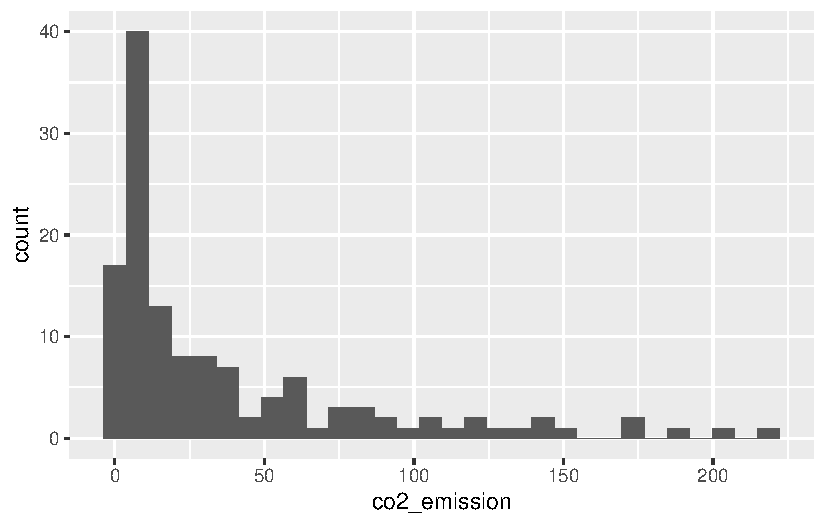
\includegraphics{intro_files/figure-pdf/unnamed-chunk-15-1.pdf}

}

\end{figure}

Mire el histograma para el arroz (rice) que acabamos de calcular. ¿Cuál
de los siguientes terminos describe mejor los datos?

\begin{itemize}
\item
  Sin sesgo
\item
  Sesgado a la izquierda
\item
  Sesgado a la derecha
\end{itemize}

Viendo el gráfico, claramento los datos están sesgado a la derecha.

En este mismo ejercicio hagamos algo más. Filtremos
\texttt{food\_consumption} para obtener las filas donde
\texttt{food\_category} está \texttt{rice}.

Luego, resumiremos los datos para obtener la media y la mediana de
\texttt{co2\_emission}, llamándolos \texttt{mean\_co2} y
\texttt{median\_co2}.

\begin{Shaded}
\begin{Highlighting}[]
\NormalTok{food\_consumption }\SpecialCharTok{\%\textgreater{}\%}
  \CommentTok{\# Filtramos por categoría de alimentos de arroz}
  \FunctionTok{filter}\NormalTok{(food\_category }\SpecialCharTok{==} \StringTok{"rice"}\NormalTok{) }\SpecialCharTok{\%\textgreater{}\%} 
  \CommentTok{\# obtenemos mean\_co2 and median\_co2}
  \FunctionTok{summarize}\NormalTok{(}\AttributeTok{mean\_co2 =} \FunctionTok{mean}\NormalTok{(co2\_emission),}
            \AttributeTok{median\_co2 =} \FunctionTok{median}\NormalTok{(co2\_emission))}
\end{Highlighting}
\end{Shaded}

\begin{verbatim}
# A tibble: 1 x 2
  mean_co2 median_co2
     <dbl>      <dbl>
1     37.6       15.2
\end{verbatim}

Dada la asimetría de estos datos, ¿Qué medida de tendencia central
resume mejor los kilogramos de \(CO_2\) emisiones por persona por año
para el arroz?

\begin{itemize}
\item
  Media
\item
  Mediana
\item
  Ambos la media y la mediana
\end{itemize}

Viendo la asimetría de los datos de nuestro último histograma, la medida
de tendencia central que mejor resume los kilogramos de CO2 emisiones
por persona será o es la mediana.

\hypertarget{medidas-de-propagaciuxf3n}{%
\section{Medidas de Propagación}\label{medidas-de-propagaciuxf3n}}

En esta sección, hablaremos sobre otro conjunto de estadísticas
resumidas: Medidas de propagación.

\hypertarget{quuxe9-es-spread}{%
\subsection{¿Qué es Spread?}\label{quuxe9-es-spread}}

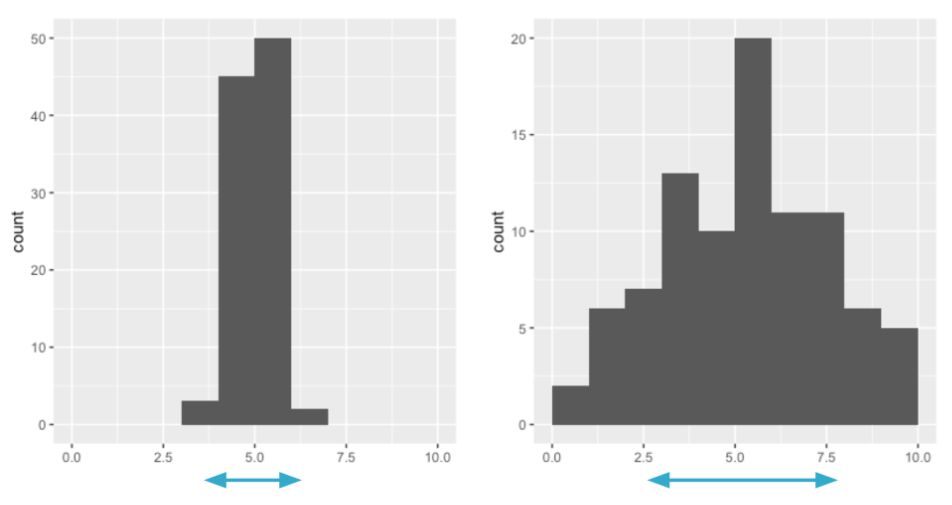
\includegraphics{fig8.png}

Spread es exactamente lo que parece: describe que tan separados o cerca
están los puntos de datos. Al igual que las medias del centro, hay
algunas medidas diferentes de extensión.

\hypertarget{la-varianza}{%
\subsection{La Varianza}\label{la-varianza}}

La primera medida, la varianza, mide la distancia promedio desde cada
punto de datos hasta la media de los datos.

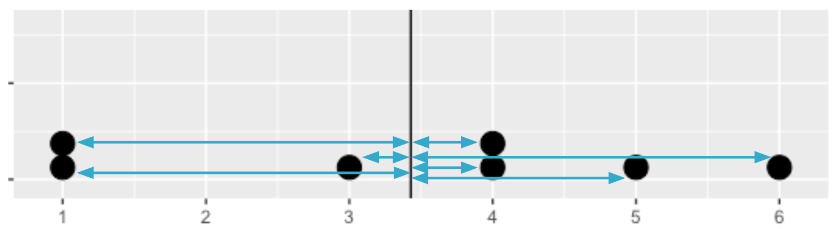
\includegraphics{fig9.png}

Para calcular la varianza, comenzamos calculando la distancia entre cada
punto y la media, por lo que obtenemos un número para cada punto de
datos.

\begin{Shaded}
\begin{Highlighting}[]
\NormalTok{dists }\OtherTok{\textless{}{-}}\NormalTok{ msleep}\SpecialCharTok{$}\NormalTok{sleep\_total }\SpecialCharTok{{-}} \FunctionTok{mean}\NormalTok{(msleep}\SpecialCharTok{$}\NormalTok{sleep\_total)}
\NormalTok{dists}
\end{Highlighting}
\end{Shaded}

\begin{verbatim}
 [1]  1.66626506  6.56626506  3.96626506  4.46626506 -6.43373494  3.96626506
 [7] -1.73373494 -3.43373494 -0.33373494 -7.43373494 -5.13373494 -1.03373494
[13] -0.43373494  2.06626506 -0.13373494 -2.13373494 -1.33373494  6.96626506
[19] -5.13373494  7.56626506 -6.53373494  9.26626506 -7.53373494 -7.33373494
[25] -0.33373494  0.46626506  4.46626506  2.06626506 -0.63373494 -8.53373494
[31] -7.73373494 -4.23373494 -4.13373494 -2.43373494 -0.93373494 -7.13373494
[37]  8.96626506 -0.33373494  3.76626506  3.86626506  2.36626506  2.06626506
[43]  9.46626506  4.16626506  0.56626506 -2.73373494  4.06626506 -2.03373494
[49] -6.63373494 -0.73373494  5.36626506 -0.03373494  3.06626506 -1.03373494
[55] -0.13373494  0.56626506  1.06626506  3.26626506 -6.93373494 -4.83373494
[61]  0.66626506  7.66626506 -5.03373494  2.56626506 -1.73373494 -0.83373494
[67] -2.03373494  0.86626506  0.16626506  6.16626506  3.36626506  5.46626506
[73]  2.36626506 -1.33373494 -1.83373494  5.36626506 -6.03373494  5.16626506
[79] -1.53373494 -5.23373494 -4.13373494  2.06626506 -0.63373494
\end{verbatim}

Luego elevamos al cuadrado cada distancia y luego las sumamos todas
juntasd.

\begin{Shaded}
\begin{Highlighting}[]
\NormalTok{squared\_dists }\OtherTok{\textless{}{-}}\NormalTok{ (dists)}\SpecialCharTok{\^{}}\DecValTok{2}
\NormalTok{squared\_dists}
\end{Highlighting}
\end{Shaded}

\begin{verbatim}
 [1]  2.776439251 43.115836841 15.731258528 19.947523588 41.392945275
 [6] 15.731258528  3.005836841 11.790535637  0.111379010 55.260415155
[11] 26.355234432  1.068607926  0.188125998  4.269451299  0.017885034
[16]  4.552824793  1.778848890 48.528848890 26.355234432 57.248366962
[21] 42.689692263 85.863668167 56.757162143 53.783668167  0.111379010
[26]  0.217403106 19.947523588  4.269451299  0.401619974 72.824632022
[31] 59.810656118 17.924511540 17.087764552  5.923065757  0.871860938
[36] 50.890174191 80.393909130  0.111379010 14.184752504 14.948005516
[41]  5.599210335  4.269451299 89.610174191 17.357764552  0.320656118
[46]  7.473306721 16.534511540  4.136077805 44.006439251  0.538366962
[51] 28.796800697  0.001138046  9.401981420  1.068607926  0.017885034
[56]  0.320656118  1.136921179 10.668487444 48.076680215 23.364993468
[61]  0.443909130 58.771619974 25.338487444  6.585716359  3.005836841
[66]  0.695113950  4.136077805  0.750415155  0.027644070 38.022824793
[71] 11.331740456 29.880053709  5.599210335  1.778848890  3.362583829
[76] 28.796800697 36.405957323 26.690294673  2.352342865 27.391981420
[81] 17.087764552  4.269451299  0.401619974
\end{verbatim}

Finalmente, dividimos la suma de las distancias al cuadrado por el
número de puntos de datos menos 1, lo que nos da la varianza.

\begin{Shaded}
\begin{Highlighting}[]
\NormalTok{sum\_sq\_dists }\OtherTok{\textless{}{-}} \FunctionTok{sum}\NormalTok{(squared\_dists)}
\NormalTok{sum\_sq\_dists}
\end{Highlighting}
\end{Shaded}

\begin{verbatim}
[1] 1624.066
\end{verbatim}

Cuanto mayor es la varianza, más dispersos están los datos. Es
importante tener en cuenta que las unidades de varianza están al
cuadrado, por lo que en este caso son 19.8 horas al cuadrado.

\begin{Shaded}
\begin{Highlighting}[]
\NormalTok{sum\_sq\_dists}\SpecialCharTok{/}\DecValTok{82}
\end{Highlighting}
\end{Shaded}

\begin{verbatim}
[1] 19.80568
\end{verbatim}

\hfill\break
Podemos calcular la varianza en un solo paso usando la función
\texttt{var} de R.

\begin{Shaded}
\begin{Highlighting}[]
\FunctionTok{var}\NormalTok{(msleep}\SpecialCharTok{$}\NormalTok{sleep\_total)}
\end{Highlighting}
\end{Shaded}

\begin{verbatim}
[1] 19.80568
\end{verbatim}

\hypertarget{desviaciuxf3n-estuxe1ndar}{%
\section{Desviación Estándar}\label{desviaciuxf3n-estuxe1ndar}}

La desviación estándar es otra medida de dispersión, calculada tomando
la raíz cuadrada de la varianza. En R se usa la función \texttt{std}
para su obtención. Lo bueno de la desviación estándar es que las
unidades suelen ser más faciles de entender ya que no están elevadas al
cuadrado. Es mejor pensar en 4 horas y media que en 19.8 horas al
cuadrado.

\begin{Shaded}
\begin{Highlighting}[]
\FunctionTok{sd}\NormalTok{(msleep}\SpecialCharTok{$}\NormalTok{sleep\_total)}
\end{Highlighting}
\end{Shaded}

\begin{verbatim}
[1] 4.450357
\end{verbatim}

\hypertarget{desviaciuxf3n-absoluta-media}{%
\subsection{Desviación Absoluta
Media}\label{desviaciuxf3n-absoluta-media}}

La desviación absoluta media toma el valor absoluto de las distancias a
la media y luego toma la media de esas diferencias. Si bien esto es
similar a la desviación estándar, no es exactamente lo mismo. La
desviación estándar eleva al cuadrado las distancias, por lo que las
distancias más largas penalizan más que las más cortas, mientras que la
desviación media absoluta penaliza cada distancia por igual. Uno no es
mejor que el otro, pero \texttt{sd} es más común que \texttt{mad}.

\begin{Shaded}
\begin{Highlighting}[]
\NormalTok{dists }\OtherTok{\textless{}{-}}\NormalTok{ msleep}\SpecialCharTok{$}\NormalTok{sleep\_total }\SpecialCharTok{{-}} \FunctionTok{mean}\NormalTok{(msleep}\SpecialCharTok{$}\NormalTok{sleep\_total)}
\FunctionTok{mean}\NormalTok{(}\FunctionTok{abs}\NormalTok{(dists))}
\end{Highlighting}
\end{Shaded}

\begin{verbatim}
[1] 3.566701
\end{verbatim}

\hypertarget{cuartiles}{%
\subsection{Cuartiles}\label{cuartiles}}

Antes de discutir la siguiente medida de dispersión, hablemos
rapidamente sobre los cuartiles. Los cuartiles dividen los datos en
cuatro partes iguales. Aquí llamamos a la función \texttt{quantile()}
para obtener los cuartiles de los datos.

\begin{Shaded}
\begin{Highlighting}[]
\FunctionTok{quantile}\NormalTok{(msleep}\SpecialCharTok{$}\NormalTok{sleep\_total)}
\end{Highlighting}
\end{Shaded}

\begin{verbatim}
   0%   25%   50%   75%  100% 
 1.90  7.85 10.10 13.75 19.90 
\end{verbatim}

Esto significa que el 25\% de los datos estan entre 1.9 y 7.85, otro
25\% de los datos está entre 7.85 y 10.10, y así sucesivamente. Esto
significa que el segundo cuartil divide los datos en dos, con el 50\% de
los datos debajo y el 50\% de los datos, arriba, por lo que es
exactamente igual que la mediana.

\hypertarget{gruxe1ficas-de-caja-usan-cuartiles}{%
\subsection{Gráficas de caja usan
cuartiles}\label{gruxe1ficas-de-caja-usan-cuartiles}}

Las cajas en los diagramas de cajas representan cuartiles. La parte
inferior de la caja es el primer cuartil y la parte superior de la caja
es el tercer cuartil. La linea media es el segundo cuartil, o la
mediana.

\begin{Shaded}
\begin{Highlighting}[]
\FunctionTok{ggplot}\NormalTok{(msleep, }\FunctionTok{aes}\NormalTok{(}\AttributeTok{y =}\NormalTok{ sleep\_total)) }\SpecialCharTok{+} 
  \FunctionTok{geom\_boxplot}\NormalTok{()}
\end{Highlighting}
\end{Shaded}

\begin{figure}[H]

{\centering 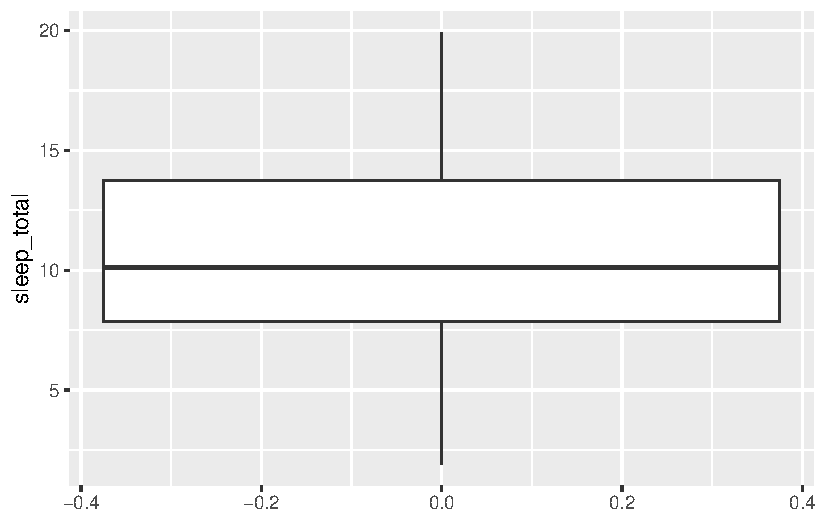
\includegraphics{intro_files/figure-pdf/unnamed-chunk-25-1.pdf}

}

\end{figure}

\hypertarget{cuantiles}{%
\subsection{Cuantiles}\label{cuantiles}}

Los cuantiles, también llamados percentiles, son una versión
generalizada del cuartil, por lo que pueden dividir los datos en 5
partes o diez partes, por ejemplo. De forma predeterminada la función
quantile devuelve los cuartiles de los datos, pero podemos ajustar esto
usando el argumento \texttt{probs} , que toma un vector de proporciones.

\begin{Shaded}
\begin{Highlighting}[]
\FunctionTok{quantile}\NormalTok{(msleep}\SpecialCharTok{$}\NormalTok{sleep\_total, }\AttributeTok{probs =} \FunctionTok{c}\NormalTok{(}\DecValTok{0}\NormalTok{, }\FloatTok{0.2}\NormalTok{, }\FloatTok{0.4}\NormalTok{, }\FloatTok{0.6}\NormalTok{, }\FloatTok{0.8}\NormalTok{, }\DecValTok{1}\NormalTok{))}
\end{Highlighting}
\end{Shaded}

\begin{verbatim}
   0%   20%   40%   60%   80%  100% 
 1.90  6.24  9.48 11.14 14.40 19.90 
\end{verbatim}

Aquí, dividimos los datos en cinco partes iguales. También podemos usar
la función \texttt{seq(from,\ to,\ by)} como atajo, que toma el número
más bajo, el número más alto y el número por el que queremos saltar.
Podemos calcular los mismos cuantiles usando \texttt{seq} de cero a uno,
saltando de 0.2.

\begin{Shaded}
\begin{Highlighting}[]
\FunctionTok{quantile}\NormalTok{(msleep}\SpecialCharTok{$}\NormalTok{sleep\_total, }\AttributeTok{probs =} \FunctionTok{seq}\NormalTok{(}\DecValTok{0}\NormalTok{, }\DecValTok{1}\NormalTok{, }\AttributeTok{by =} \FloatTok{0.2}\NormalTok{))}
\end{Highlighting}
\end{Shaded}

\begin{verbatim}
   0%   20%   40%   60%   80%  100% 
 1.90  6.24  9.48 11.14 14.40 19.90 
\end{verbatim}

\hypertarget{rango-intercuartilico-iqr}{%
\section{Rango Intercuartilico (IQR)}\label{rango-intercuartilico-iqr}}

El rango intercuartilico, o IQR, es otra medida de dispersión. Es la
distancia entre los percentiles 25 y 75 que también es la altura de la
caja en un diagrama de caja. Podemos calcularlo usando la función
cuantil para obtener 5.9 horas.

\begin{Shaded}
\begin{Highlighting}[]
\FunctionTok{quantile}\NormalTok{(msleep}\SpecialCharTok{$}\NormalTok{sleep\_total, }\FloatTok{0.75}\NormalTok{) }\SpecialCharTok{{-}} \FunctionTok{quantile}\NormalTok{(msleep}\SpecialCharTok{$}\NormalTok{sleep\_total, }\FloatTok{0.25}\NormalTok{)}
\end{Highlighting}
\end{Shaded}

\begin{verbatim}
75% 
5.9 
\end{verbatim}

\hypertarget{valores-atuxedpicos}{%
\subsection{Valores atípicos}\label{valores-atuxedpicos}}

Los valores atípicos son puntos de datos que son sustancialmente
diferentes de los demás. Pero, ¿cómo sabemos qué es una diferencia
sustancial? Una regla que se usa a menudo es que cualquier punto de
datos menor que el primer cuartil menos 1.5 veces el IQR es un valor
atípico. Así como cualquier punto mayor que el tercer cuartil más 1.5
veces el IQR.

\begin{itemize}
\item
  \(data < Q_1 - 1.5\times IQR\)
\item
  \(data > Q_3 + 1.5\times IQR\)
\end{itemize}

\hypertarget{encontrar-valores-atuxedpicos}{%
\subsection{Encontrar valores
atípicos}\label{encontrar-valores-atuxedpicos}}

Para encontrar valores atípicos, comenzaremos calculando el IQR de los
pesos corporales de los mamiferos.

\begin{Shaded}
\begin{Highlighting}[]
\NormalTok{iqr }\OtherTok{\textless{}{-}} \FunctionTok{quantile}\NormalTok{(msleep}\SpecialCharTok{$}\NormalTok{sleep\_total,}\FloatTok{0.75}\NormalTok{) }\SpecialCharTok{{-}} \FunctionTok{quantile}\NormalTok{(msleep}\SpecialCharTok{$}\NormalTok{sleep\_total, }\FloatTok{0.25}\NormalTok{)}
\end{Highlighting}
\end{Shaded}

Luego podemos calcular los umbrales inferior y superior siguiendo las
fórmulas de la diapositiva anterior.

\begin{Shaded}
\begin{Highlighting}[]
\NormalTok{lower\_threshold }\OtherTok{\textless{}{-}} \FunctionTok{quantile}\NormalTok{(msleep}\SpecialCharTok{$}\NormalTok{sleep\_total, }\FloatTok{0.25}\NormalTok{) }\SpecialCharTok{{-}} \FloatTok{1.5}\SpecialCharTok{*}\NormalTok{iqr}
\NormalTok{upper\_threshold }\OtherTok{\textless{}{-}} \FunctionTok{quantile}\NormalTok{(msleep}\SpecialCharTok{$}\NormalTok{sleep\_total, }\FloatTok{0.75}\NormalTok{) }\SpecialCharTok{+} \FloatTok{1.5}\SpecialCharTok{*}\NormalTok{iqr}
\end{Highlighting}
\end{Shaded}

Ahora podemos filtrar el marco de datos para encontrar mamiferos cuyo
peso corporal esta por encima o por debajo de los umbrales.

\begin{Shaded}
\begin{Highlighting}[]
\NormalTok{msleep }\SpecialCharTok{\%\textgreater{}\%} \FunctionTok{filter}\NormalTok{(bodywt }\SpecialCharTok{\textless{}}\NormalTok{ lower\_threshold }\SpecialCharTok{|}\NormalTok{ bodywt }\SpecialCharTok{\textgreater{}}\NormalTok{ upper\_threshold) }\SpecialCharTok{\%\textgreater{}\%} 
  \FunctionTok{select}\NormalTok{(name, vore, sleep\_total, bodywt)}
\end{Highlighting}
\end{Shaded}

\begin{verbatim}
# A tibble: 23 x 4
   name           vore  sleep_total bodywt
   <chr>          <chr>       <dbl>  <dbl>
 1 Cheetah        carni        12.1   50  
 2 Cow            herbi         4    600  
 3 Goat           herbi         5.3   33.5
 4 Asian elephant herbi         3.9 2547  
 5 Horse          herbi         2.9  521  
 6 Donkey         herbi         3.1  187  
 7 Giraffe        herbi         1.9  900. 
 8 Pilot whale    carni         2.7  800  
 9 Gray seal      carni         6.2   85  
10 Human          omni          8     62  
# i 13 more rows
\end{verbatim}

Podemos ver que hay 23 valores atípicos de peso corporal en este
conjunto de datos, incluidos la vaca y el elefante asiático.

\hypertarget{ejercicio-3}{%
\section{Ejercicio 3}\label{ejercicio-3}}

Los cuantiles ya sabemos que son una excelente manera de resumir datos
numéricos, ya que se pueden usar para medir el centro y la dispersión,
así como para tener una idea de dónde se encuentra un punto de datos en
relación con el resto del conjunto de datos. Por ejemplo, es posible que
desee otorgar un descuento al 10\% de los usuarios más activos en un
sitio web.

En este ejercicio, calculará cuartiles, quantiles y deciles, que dividen
un conjunto de datos en 4, 5 y 10 partes, respectivamente.

Primero calculemos los cuartiles de la columna \texttt{co2\_emssion} de
\texttt{food\_consumption}.

\begin{Shaded}
\begin{Highlighting}[]
\FunctionTok{quantile}\NormalTok{(food\_consumption}\SpecialCharTok{$}\NormalTok{co2\_emission)}
\end{Highlighting}
\end{Shaded}

\begin{verbatim}
       0%       25%       50%       75%      100% 
   0.0000    5.2100   16.5300   62.5975 1712.0000 
\end{verbatim}

Calculamos ahora, los seis cuantiles que dividen los datos en 5 partes
(quantiles) de la columna \texttt{co2\_emission} de
\texttt{food\_consumption}.

\begin{Shaded}
\begin{Highlighting}[]
\FunctionTok{quantile}\NormalTok{(food\_consumption}\SpecialCharTok{$}\NormalTok{co2\_emission, }\AttributeTok{probs =} \FunctionTok{seq}\NormalTok{(}\DecValTok{0}\NormalTok{,}\DecValTok{1}\NormalTok{,}\FloatTok{0.2}\NormalTok{))}
\end{Highlighting}
\end{Shaded}

\begin{verbatim}
      0%      20%      40%      60%      80%     100% 
   0.000    3.540   11.026   25.590   99.978 1712.000 
\end{verbatim}

Por último, calculamos los once cuantiles de \texttt{co2\_emission} esa
división de los datos en diez partes (deciles).

\begin{Shaded}
\begin{Highlighting}[]
\FunctionTok{quantile}\NormalTok{(food\_consumption}\SpecialCharTok{$}\NormalTok{co2\_emission, }\AttributeTok{probs =} \FunctionTok{seq}\NormalTok{(}\DecValTok{0}\NormalTok{,}\DecValTok{1}\NormalTok{,}\FloatTok{0.1}\NormalTok{))}
\end{Highlighting}
\end{Shaded}

\begin{verbatim}
      0%      10%      20%      30%      40%      50%      60%      70% 
   0.000    0.668    3.540    7.040   11.026   16.530   25.590   44.271 
     80%      90%     100% 
  99.978  203.629 1712.000 
\end{verbatim}

\hypertarget{ejercicio-4}{%
\section{Ejercicio 4}\label{ejercicio-4}}

Ya vio previamente que la varianza y la desviación estándar son dos de
las formas más comunes de medir la dispersión de una variable, y
practicaremos su cálculo en este ejercicio. La difusión es importante ya
que puede ayudar a informar las expectativas. Por ejemplo, si un
vendedor vende una media de 20 productos al día, pero tiene una
desviación estándar de 10 productos, probablemente habrá días en los que
solo venderá uno o dos. Información como esta es importante,
especialmente cuando se hacen predicciones.

Para este ejericio, primer calcularemos la varianza y la desviación
estándar de \texttt{co2\_emission} para cada una de las
\texttt{food\_category} agrupando por y resumiendo la varianza como
\texttt{var\_co2} y la desviación estándar como \texttt{sd\_co2}.

\begin{Shaded}
\begin{Highlighting}[]
\NormalTok{food\_consumption }\SpecialCharTok{\%\textgreater{}\%} 
  \FunctionTok{group\_by}\NormalTok{(food\_category) }\SpecialCharTok{\%\textgreater{}\%} 
  \FunctionTok{summarize}\NormalTok{(}\AttributeTok{var\_co2 =} \FunctionTok{var}\NormalTok{(co2\_emission),}
           \AttributeTok{sd\_co2 =} \FunctionTok{sd}\NormalTok{(co2\_emission))}
\end{Highlighting}
\end{Shaded}

\begin{verbatim}
# A tibble: 11 x 3
   food_category   var_co2  sd_co2
   <fct>             <dbl>   <dbl>
 1 beef          88748.    298.   
 2 eggs             21.4     4.62 
 3 fish            922.     30.4  
 4 lamb_goat     16476.    128.   
 5 dairy         17672.    133.   
 6 nuts             35.6     5.97 
 7 pork           3095.     55.6  
 8 poultry         245.     15.7  
 9 rice           2281.     47.8  
10 soybeans          0.880   0.938
11 wheat            71.0     8.43 
\end{verbatim}

Luego, creemos un histograma de \texttt{co2\_emission} para cada una de
\texttt{food\_category} usando \texttt{facet\_wrap()}.

\begin{Shaded}
\begin{Highlighting}[]
\FunctionTok{library}\NormalTok{(ggplot2)}
\FunctionTok{ggplot}\NormalTok{(food\_consumption, }\FunctionTok{aes}\NormalTok{(co2\_emission)) }\SpecialCharTok{+}
  \CommentTok{\# Creación del  histograma}
  \FunctionTok{geom\_histogram}\NormalTok{() }\SpecialCharTok{+}
  \CommentTok{\# Creamos subgráficos separados para cada categoría de food\_category}
  \FunctionTok{facet\_wrap}\NormalTok{(}\SpecialCharTok{\textasciitilde{}}\NormalTok{ food\_category)}
\end{Highlighting}
\end{Shaded}

\begin{verbatim}
`stat_bin()` using `bins = 30`. Pick better value with `binwidth`.
\end{verbatim}

\begin{figure}[H]

{\centering 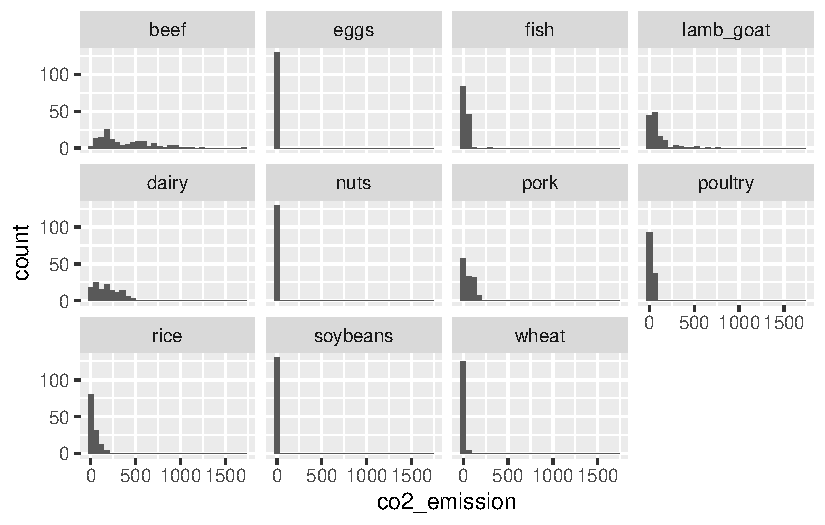
\includegraphics{intro_files/figure-pdf/unnamed-chunk-36-1.pdf}

}

\end{figure}

Excelente medición de dispersión! La carne de res tiene la mayor
cantidad de variación en sus emisiones de CO2, mientras que los huevos,
las nueces y la soya tienen cantidades relativamente pequeñas de
variación.

\hypertarget{ejercicio-5}{%
\section{Ejercicio 5}\label{ejercicio-5}}

Los valores atípicos pueden tener grandes efectos en las estadísticas
como la media, así como en las estadísticas que se basan en la media,
como la varianza y la desviación estándar. El rango intercuartilico, o
IQR, es otra forma de medir la dispersión que está menos influenciada
por los valores atípicos. IQR también se usa a menudo para encontrar
valores atípicos. Si un valor es menor que \(Q_1 - 1.5\times IQR\) o
mayor que \(Q_3 + 1.5\times IQR\), se considera un valor atípico. De
hecho, así es como \texttt{ggplot2} se calculan las longitudes de los
bigotes en un diagrama de caja.

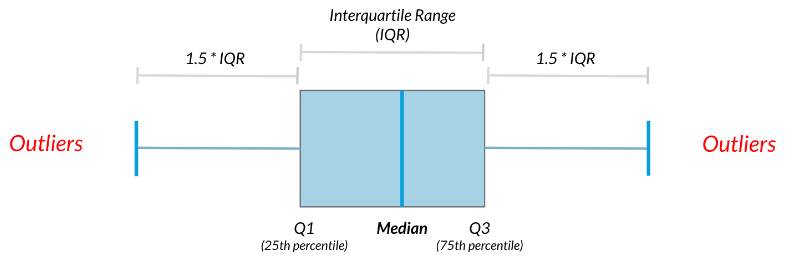
\includegraphics{fig10.png}

En este ejercicio, calcularemos IQR y lo utilizaremos para encontrar
algunos valores atípicos.

Primero calculamos el total de \texttt{co2\_emission} por país agrupando
por país y tomando la suma de \texttt{co2\_emission}. Llamaremos a la
suma \texttt{total\_emission} y almacenaremos el marco de datos
resultante como \texttt{emission\_by\_country}.

\begin{Shaded}
\begin{Highlighting}[]
\FunctionTok{library}\NormalTok{(tidyverse)}

\NormalTok{emissions\_by\_country }\OtherTok{\textless{}{-}}\NormalTok{ food\_consumption }\SpecialCharTok{\%\textgreater{}\%}
  \FunctionTok{group\_by}\NormalTok{(country) }\SpecialCharTok{\%\textgreater{}\%}
  \FunctionTok{summarize}\NormalTok{(}\AttributeTok{total\_emission =} \FunctionTok{sum}\NormalTok{(co2\_emission))}

\NormalTok{emissions\_by\_country }\SpecialCharTok{\%\textgreater{}\%}
  \FunctionTok{head}\NormalTok{()}
\end{Highlighting}
\end{Shaded}

\begin{verbatim}
# A tibble: 6 x 2
  country   total_emission
  <chr>              <dbl>
1 Albania            1778.
2 Algeria             708.
3 Angola              413.
4 Argentina          2172.
5 Armenia            1110.
6 Australia          1939.
\end{verbatim}

Ahora, calcularemos el primer y tercer cuartil de
\texttt{total\_emission} y lo guardamos como \texttt{q1} y \texttt{q3}.

\begin{Shaded}
\begin{Highlighting}[]
\NormalTok{q1 }\OtherTok{\textless{}{-}} \FunctionTok{quantile}\NormalTok{(emissions\_by\_country}\SpecialCharTok{$}\NormalTok{total\_emission, }\FloatTok{0.25}\NormalTok{)}
\NormalTok{q3 }\OtherTok{\textless{}{-}} \FunctionTok{quantile}\NormalTok{(emissions\_by\_country}\SpecialCharTok{$}\NormalTok{total\_emission, }\FloatTok{0.75}\NormalTok{)}
\NormalTok{iqr }\OtherTok{\textless{}{-}}\NormalTok{ q3}\SpecialCharTok{{-}}\NormalTok{q1}
\end{Highlighting}
\end{Shaded}

Luego, calculamos los puntos de corto inferior y superior para los
valores atípicos de \texttt{total\_emission} y guardamos como
\texttt{lower} y \texttt{upper}.

\begin{Shaded}
\begin{Highlighting}[]
\NormalTok{lower }\OtherTok{\textless{}{-}}\NormalTok{ q1}\FloatTok{{-}1.5}\SpecialCharTok{*}\NormalTok{iqr}
\NormalTok{upper }\OtherTok{\textless{}{-}}\NormalTok{ q3}\FloatTok{+1.5}\SpecialCharTok{*}\NormalTok{iqr}
\end{Highlighting}
\end{Shaded}

Usamos \texttt{filter()} para obtener países con un límite
\texttt{total\_emission} superior o inferior al límite. \texttt{upper}
\texttt{total\_emission} \texttt{lower}.

\begin{Shaded}
\begin{Highlighting}[]
\NormalTok{emissions\_by\_country }\SpecialCharTok{\%\textgreater{}\%}
  \FunctionTok{filter}\NormalTok{(total\_emission }\SpecialCharTok{\textless{}}\NormalTok{ lower }\SpecialCharTok{|}\NormalTok{ total\_emission }\SpecialCharTok{\textgreater{}}\NormalTok{ upper)}
\end{Highlighting}
\end{Shaded}

\begin{verbatim}
# A tibble: 1 x 2
  country   total_emission
  <chr>              <dbl>
1 Argentina          2172.
\end{verbatim}

Como puede ver, parece que Argentina tiene una cantidad sustancialmente
mayor de emisiones de CO2 por persona que otros países del mundo.

\bookmarksetup{startatroot}

\hypertarget{nuxfameros-aleatorios-y-probabilidad}{%
\chapter{Números aleatorios y
Probabilidad}\label{nuxfameros-aleatorios-y-probabilidad}}

En este capítulo, aprenderá cómo generar muestras aleatorias y medir al
azar usando la probabilidad. Trabajara con datos de ventas del mundo
real para calcular la probabilidad de que un vendedor tenga éxito.
Finalmente, utilizará la distribución binomial para modelar los eventos
con resultados binarios.

\hypertarget{quuxe9-son-las-probabilidades}{%
\section{¿Qué son las
probabilidades?}\label{quuxe9-son-las-probabilidades}}

La gente habla de suerte con bastante frecuencia, como ¿cuales son las
posibilidades de cerrar una venta, de que llueva mañana o de ganar un
juego? Pero, ¿Cómo medimos exactamente el azar?

Podemos medir las probabilidades o posibilidades de un evento usando la
probabilidad. Podemos calcular la probabilidad de ocurrencia de un
evento tomando el número de formas en que el evento puede suceder
dividiéndolo por el número total de resultados posibiles.

\[
P(Evento) = \frac{\mbox{\# de formas en que puede ocurrir el evento}}{\mbox{\# total de resultados posibles}}
\]

Por ejemplo, si lanzamos una moneda, puede caer en cara o cruz. Para
obtener la probabilidad de que la moneda caiga en cara, dividimos la
forma de obtener cara entre los dos resultados posibles, cara y cruz.

\[
P(cara) = \frac{\mbox{1 forma de obtener cara}}{\mbox{2 posibles resultados}} = \frac{1}{2} = fbox{50\%}
\]

La probabilidad siempre está entte cero y 100\% por ciento. Si la
probabilidad de algo es cero, es imposible, y si la probabilidad de algo
es del 100\%, ciertamente sucederá.

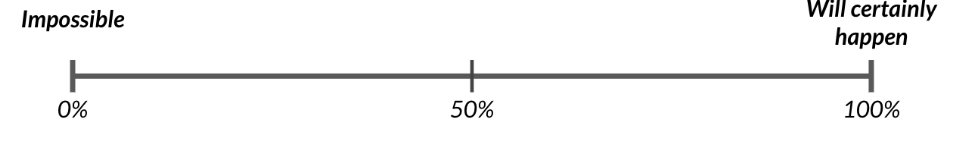
\includegraphics{fig11.png}

\hypertarget{asisgnaciuxf3n-de-vendedores}{%
\section{Asisgnación de Vendedores}\label{asisgnaciuxf3n-de-vendedores}}

Veamos un escenaro más complejo. Se acerca una reunión con un cliente
potencial y queremos enviar a alguien del equipo de ventas a la reunión.
Pondremos el nombre de cada persona en un boleto en una caja y sacaremos
uno al azar para decidir quién va a reunión.

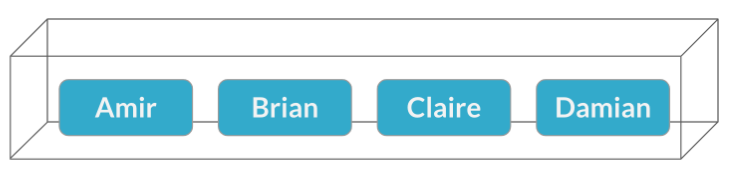
\includegraphics{fig12.png}

El nombre de Brian se saca.

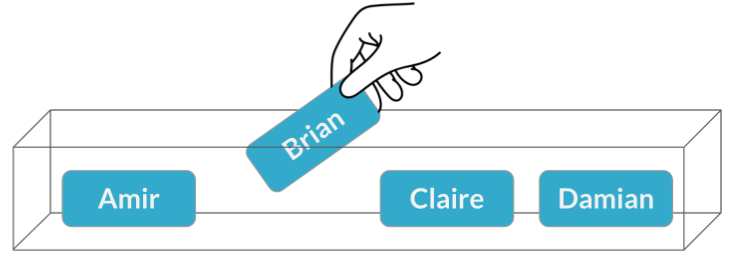
\includegraphics{fig13.png}

La probabilidad de que Brian sea seleccionado es una de cuatro, o 25\%.
Esto es

\[
P(Brian) = \frac{1}{4} = \fbox{25%}
\]

\hypertarget{muestreo-desde-un-marco-de-datos}{%
\subsection{Muestreo desde un marco de
datos}\label{muestreo-desde-un-marco-de-datos}}

Podemos recrear este escenario en R usando la función \texttt{sample\_n}
de \texttt{dplyr}, que toma un marco de datos y la cantidad de filas que
queremos extraer, que es solo 1 en este caso.

\begin{Shaded}
\begin{Highlighting}[]
\FunctionTok{library}\NormalTok{(dplyr)}
\end{Highlighting}
\end{Shaded}

\begin{verbatim}

Attaching package: 'dplyr'
\end{verbatim}

\begin{verbatim}
The following objects are masked from 'package:stats':

    filter, lag
\end{verbatim}

\begin{verbatim}
The following objects are masked from 'package:base':

    intersect, setdiff, setequal, union
\end{verbatim}

\begin{Shaded}
\begin{Highlighting}[]
\NormalTok{sales\_counts }\OtherTok{\textless{}{-}} \FunctionTok{data.frame}\NormalTok{(}\AttributeTok{name =} \FunctionTok{c}\NormalTok{(}\StringTok{"Amir"}\NormalTok{, }\StringTok{"Brian"}\NormalTok{, }\StringTok{"claire"}\NormalTok{, }\StringTok{"Damian"}\NormalTok{), }\AttributeTok{n\_sales =} \FunctionTok{c}\NormalTok{(}\DecValTok{178}\NormalTok{, }\DecValTok{126}\NormalTok{, }\DecValTok{75}\NormalTok{, }\DecValTok{69}\NormalTok{))}

\NormalTok{sales\_counts }\SpecialCharTok{\%\textgreater{}\%} 
  \FunctionTok{sample\_n}\NormalTok{(}\DecValTok{1}\NormalTok{)}
\end{Highlighting}
\end{Shaded}

\begin{verbatim}
  name n_sales
1 Amir     178
\end{verbatim}

Sin embargo, si ejecutamos lo mismo nuevamente, es posible que
obtengamos una fila diferente ya que \texttt{sample\_n} elige al azar.

\begin{Shaded}
\begin{Highlighting}[]
\NormalTok{sales\_counts }\SpecialCharTok{\%\textgreater{}\%} 
  \FunctionTok{sample\_n}\NormalTok{(}\DecValTok{1}\NormalTok{)}
\end{Highlighting}
\end{Shaded}

\begin{verbatim}
   name n_sales
1 Brian     126
\end{verbatim}

Si queremos mostrarle al aquipo cómo elegimos a Brian, esto no
funcionará bien.

\hypertarget{establecer-una-semilla-aleatoria}{%
\subsection{Establecer una semilla
aleatoria}\label{establecer-una-semilla-aleatoria}}

Para asegurarnos de obtener los mismos resultados cuando ejectuamos el
script frente al equipo, configuremos la semilla aleatoria usando
\texttt{set.seed()}. La semilla es un número que el generador de números
aleatorios de R usa como punto de partida, por lo que si lo orientamos
con un número semilla, generará el mismo valor aleatorio cada vez. El
número en si no importa. Podríamos usar 5,139 o 3 millones. Lo único que
importa es que usemos la misma semilla la próxima vez que ejecutemos el
script. Ahora, nosotros, o uno de los miembros del equipo de ventas,
podemos ejecutar este código una y otra vez y obtener el mismo resultado
de Brian cada vez.

\begin{Shaded}
\begin{Highlighting}[]
\FunctionTok{set.seed}\NormalTok{(}\DecValTok{5}\NormalTok{)}
\NormalTok{sales\_counts }\SpecialCharTok{\%\textgreater{}\%} 
  \FunctionTok{sample\_n}\NormalTok{(}\DecValTok{1}\NormalTok{)}
\end{Highlighting}
\end{Shaded}

\begin{verbatim}
   name n_sales
1 Brian     126
\end{verbatim}

\hypertarget{un-segundo-encuentro}{%
\subsection{Un segundo encuentro}\label{un-segundo-encuentro}}

Ahora hay otro cliente potencial que quiere reunirse al mismo tiempo,
por lo que debemos elegir a otro vendedor. Brian ya ha sido elegido y no
puede estar en dos reuniones a la vez, así que elegiremos entre las tres
restantes. A esto se le llama \textbf{\texttt{muestro\ sin\ reemplazo}},
ya que no estamos reemplazando el nombre que ya sacamos. Esta vez, se
elegi a Claire,

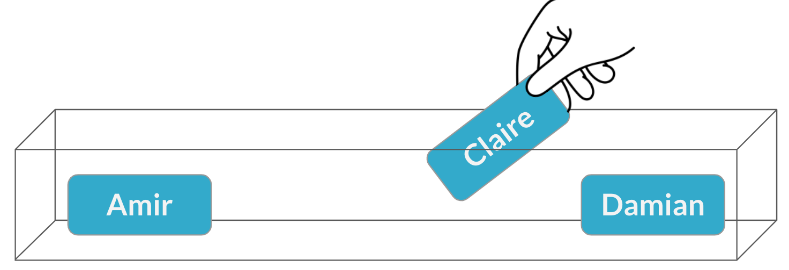
\includegraphics{fig14.png}

y la probabilidad de que estos suceda es una de cada tres, o al rededor
del 33\%. Esto es,

\[
P(Claire) = \frac{1}{3} = \fbox{33%}
\]

Para recrear esto en R, podemos pasar 2 a sample\_b, lo quie nos dará
filas.

\begin{Shaded}
\begin{Highlighting}[]
\FunctionTok{set.seed}\NormalTok{(}\DecValTok{5}\NormalTok{)}
\NormalTok{sales\_counts }\SpecialCharTok{\%\textgreater{}\%} 
  \FunctionTok{sample\_n}\NormalTok{(}\DecValTok{2}\NormalTok{)}
\end{Highlighting}
\end{Shaded}

\begin{verbatim}
    name n_sales
1  Brian     126
2 claire      75
\end{verbatim}

Ahora digamos que las dos reuniones se realizan en diás diferentes, por
lo que la misma persona podría asistir a ambas. En este escenario,
debemos devolver el nombre de Brian a la caja después de elegirla. Esto
se llama \textbf{\texttt{muestreo\ con\ reemplazo}}. Claire es elegida
para la segunda reunión

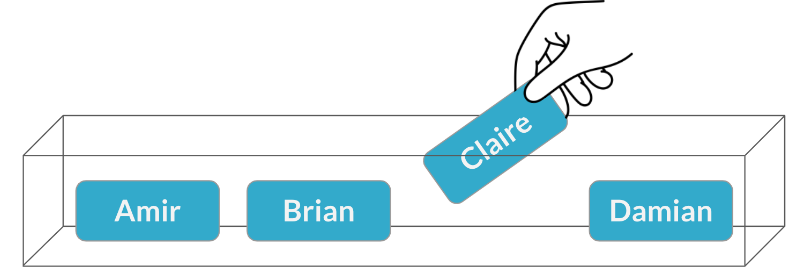
\includegraphics{fig15.png}

Pero esta vez, la probabilidad es del 25\%.

\[
P(Claire) = \frac{1}{4} = \fbox{25%}
\]

Para hacer esto en R, establezca el argumento de reemplazo de sample\_n
en \texttt{TRUE}.

\begin{Shaded}
\begin{Highlighting}[]
\FunctionTok{set.seed}\NormalTok{(}\DecValTok{5}\NormalTok{)}
\NormalTok{sales\_counts }\SpecialCharTok{\%\textgreater{}\%} 
  \FunctionTok{sample\_n}\NormalTok{(}\DecValTok{2}\NormalTok{, }\AttributeTok{replace =} \ConstantTok{TRUE}\NormalTok{)}
\end{Highlighting}
\end{Shaded}

\begin{verbatim}
    name n_sales
1  Brian     126
2 claire      75
\end{verbatim}

\hypertarget{eventos-independientes}{%
\subsection{Eventos Independientes}\label{eventos-independientes}}

Hablemos rapidamente de la independencia. Dos eventos son independientes
si la probabilidad del segundo evento no se ve afectada por el resultado
del primero. Por ejemplo, si estamos muestreando con reemplazo, la
probabilidad que Claire sea elegida en segundo lugar es del 25\%, sin
importar quien sea elegido primero. En general, al muestrear
\texttt{con\ reemplazo}, cada selección es independiente.

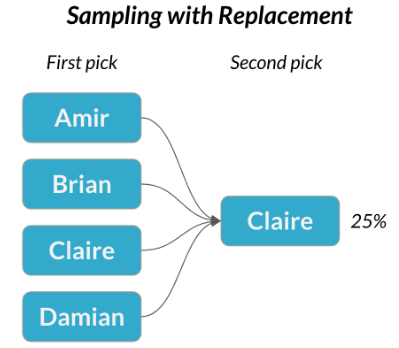
\includegraphics{fig16.png}

De manera similar, los eventos se consideran dependientes cuando el
resultado del primero cambia la probabilidad del segundo. Si muestreamos
\texttt{sin\ reemplazo}, la probabilidad de que Claire sea elegida en
segundo lugar depende de quién sea elegido primero. Si Claire es elegida
primero, hay 0\% de probabilidad de que Claire sea elegida en segundo
lugar.

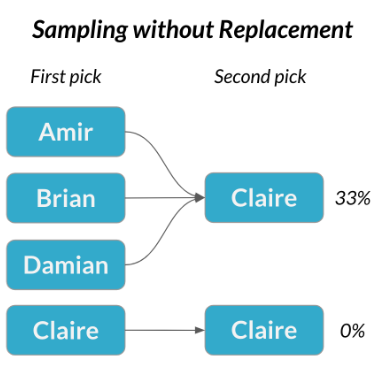
\includegraphics{fig17.png}

En general, cuando se muestrea sin reemplazo, cada selección es
dependiente.

El siguiente cuadro comparativo contiene algunos ejemplos sobre muestreo
con reemplazo y sin reemplazo.

\begin{longtable}[]{@{}
  >{\raggedright\arraybackslash}p{(\columnwidth - 2\tabcolsep) * \real{0.2500}}
  >{\raggedright\arraybackslash}p{(\columnwidth - 2\tabcolsep) * \real{0.7500}}@{}}
\toprule\noalign{}
\begin{minipage}[b]{\linewidth}\raggedright
Con Reemplazo
\end{minipage} & \begin{minipage}[b]{\linewidth}\raggedright
Sin Reemplazo
\end{minipage} \\
\midrule\noalign{}
\endhead
\bottomrule\noalign{}
\endlastfoot
Lanzar una moneda 3 veces & De una baraja de cartas, repartiendo a 3
jugadores 7 cartas cada un., \\
Tirar un dado dos veces & Seleccionar al azar 5 productos de la linea de
montaje para probar el control de calidad \\
& Elegir al azar a 3 personas para trabajar el fin de semana de un grupo
de 20 personas \\
\end{longtable}

\hypertarget{ejemplo-6}{%
\section{Ejemplo 6}\label{ejemplo-6}}

Suponga que está a cargo del equipo de ventas y es hora de realizar
revisiones de desempeño, comenzando con Amir. Como parte de la revisión,
desea seleccionar al azar algunas de las ofertas en las que ha trabajado
durante el último año para que pueda verlas más a fondo. Antes de
comenzar a seleccionar ofertas, primero averiguará cuáles son las
probabilidades de seleccionar ciertas ofertas.

La data que se creo a continuación, contiene la cantidad de tratos en
los que Amir trabajo para cada tipo de producto.

\begin{Shaded}
\begin{Highlighting}[]
\NormalTok{amir\_deals }\OtherTok{\textless{}{-}} \FunctionTok{data.frame}\NormalTok{(}\AttributeTok{product =} \FunctionTok{c}\NormalTok{(}\StringTok{"Product A"}\NormalTok{, }\StringTok{"Product B"}\NormalTok{, }\StringTok{"Product C"}\NormalTok{, }\StringTok{"Product D"}\NormalTok{, }\StringTok{"Product E"}\NormalTok{, }\StringTok{"Product F"}\NormalTok{, }\StringTok{"Product G"}\NormalTok{, }\StringTok{"Product H"}\NormalTok{, }\StringTok{"Product I"}\NormalTok{, }\StringTok{"Product J"}\NormalTok{, }\StringTok{"Product N"}\NormalTok{), }\AttributeTok{n =} \FunctionTok{c}\NormalTok{(}\DecValTok{23}\NormalTok{, }\DecValTok{62}\NormalTok{, }\DecValTok{15}\NormalTok{, }\DecValTok{40}\NormalTok{, }\DecValTok{5}\NormalTok{, }\DecValTok{11}\NormalTok{, }\DecValTok{2}\NormalTok{, }\DecValTok{8}\NormalTok{, }\DecValTok{7}\NormalTok{, }\DecValTok{2}\NormalTok{, }\DecValTok{3}\NormalTok{))}
\end{Highlighting}
\end{Shaded}

Ahora, creamos una nueva columna llamada \texttt{prob} dividiendo
\texttt{n} por el número total de tratos en los que trabajó Amir.

\begin{Shaded}
\begin{Highlighting}[]
\NormalTok{amir\_deals }\SpecialCharTok{\%\textgreater{}\%}
  \FunctionTok{mutate}\NormalTok{(}\AttributeTok{prob =}\NormalTok{ n}\SpecialCharTok{/}\FunctionTok{sum}\NormalTok{(n))}
\end{Highlighting}
\end{Shaded}

\begin{verbatim}
     product  n       prob
1  Product A 23 0.12921348
2  Product B 62 0.34831461
3  Product C 15 0.08426966
4  Product D 40 0.22471910
5  Product E  5 0.02808989
6  Product F 11 0.06179775
7  Product G  2 0.01123596
8  Product H  8 0.04494382
9  Product I  7 0.03932584
10 Product J  2 0.01123596
11 Product N  3 0.01685393
\end{verbatim}

Si selecciona al azar una de las ofertas de Amir, ¿cuál es la
probabilidad de que la oferta involucre el Producto C?

\textbf{Respuesta: 8.43\%}

\hypertarget{distribuciones-discretas}{%
\section{Distribuciones Discretas}\label{distribuciones-discretas}}

En esta lección, profundizaremos en la probabilidad y comenzaremos a
observar las distribuciones de probabilidad.

Consideremos lanzar un dado estándar de seis caras.

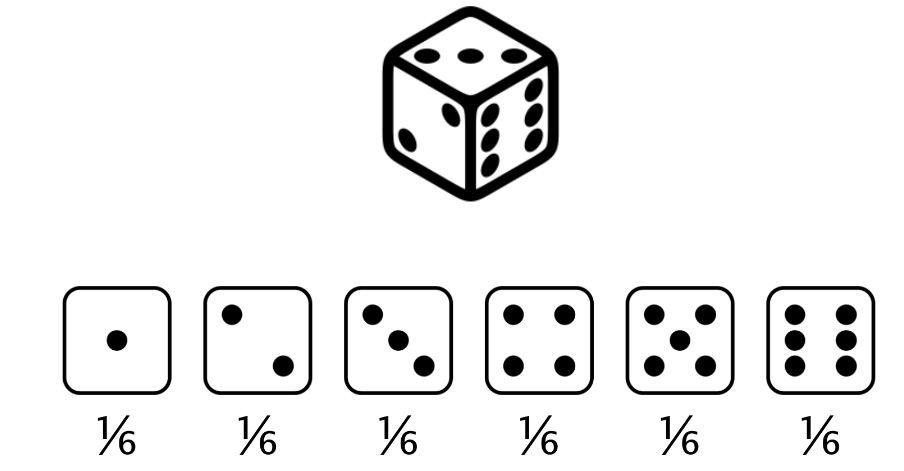
\includegraphics{fig18.png}

Hay seis números, o seis resultados posibles, y cada número tiene
exactamente una sexta parte, o alrededor de un 17 por ciento de
posibilidades de salir. Este es un ejemplo de una distribución de
probabilidad.

Esto es similar al escenario anterior, excepto que teneiamos nombres en
lugar de números.

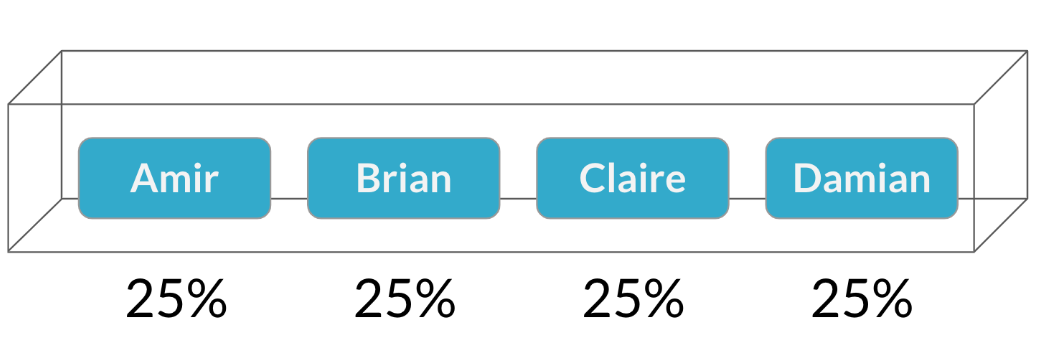
\includegraphics{fig19.png}

Al igual que tirar un dado, cada resultado o nombre tenía la misma
probabilidad de ser elegido.

\hypertarget{distribuciuxf3n-de-probabilidad}{%
\subsection{Distribución de
Probabilidad}\label{distribuciuxf3n-de-probabilidad}}

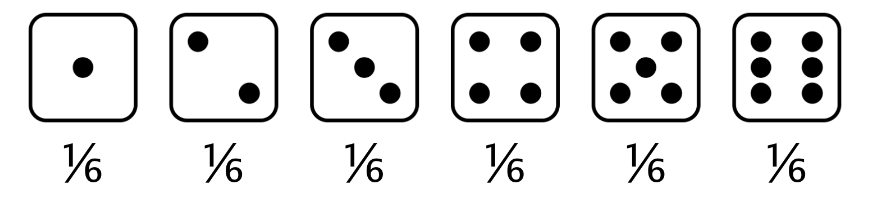
\includegraphics{fig20.png}

Una distribución de probabilidad describe la probabilidad de cada
resultado posible en un escenario.

\hypertarget{valor-esperado}{%
\subsubsection{Valor esperado}\label{valor-esperado}}

También podemos hablar del valor esperado de una distribución, que es la
media de una distribución.

Podemos calcular esto multiplicando cada valor por su probabilidad y
sumando, por lo que el valor esperado de lanzar un dado justo es 3.5. En
el caso de los dados sera:

\[
(1\times \frac{1}{6}) + (2\times \frac{1}{6}) + (3\times \frac{1}{6}) + (4\times \frac{1}{6}) + (5\times \frac{1}{6}) + (6\times \frac{1}{6}) = \fbox{3.5}
\]

Podemos visualizar esto usando un gráfico de barras, donde cada barra
representa un resultado, y la altura de cada barra representa la
probabilidad de ese resultado.

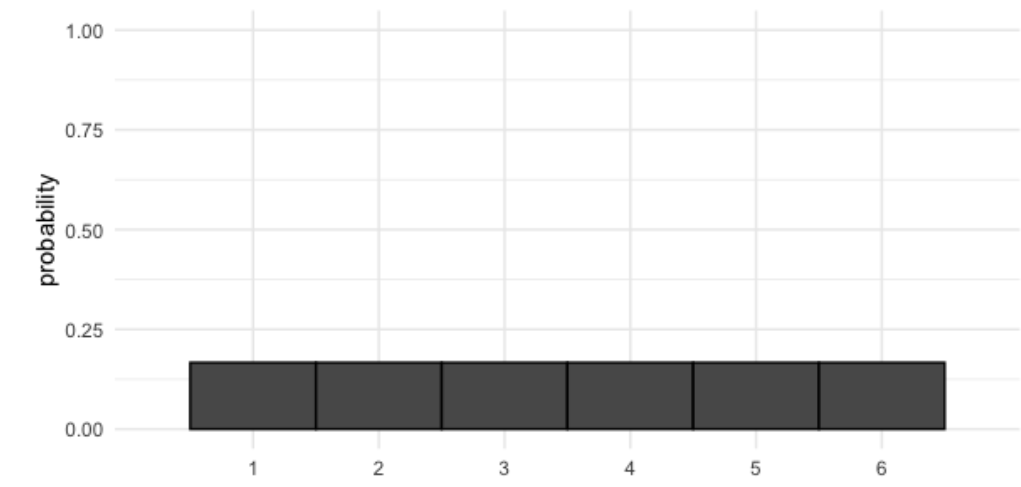
\includegraphics{fig21.png}

\hypertarget{probabilidad-uxe1rea}{%
\subsubsection{Probabilidad = área}\label{probabilidad-uxe1rea}}

Podemos calcular las probabilidades de diferentes resultados tomando
áreas de la distribución de probabilidad. Por ejemplo, ¿cuál es la
probabilidad de que nuestra tirada sea menor o igual a 2?

\[
¿P(\mbox{tirada dado}) \leq 2?
\]

Para resolver esto, tomaremos el área de cada barra que representa un
resultado de 2 o menos. Cada barra tiene un ancho de 1 y una altura de
1/6, por lo que el área de cada barra es un sexto. Sumamos las áreas de
1 y 2 como se muestra en el gráfico para obtener una probabilidad total
de \(1/3\).

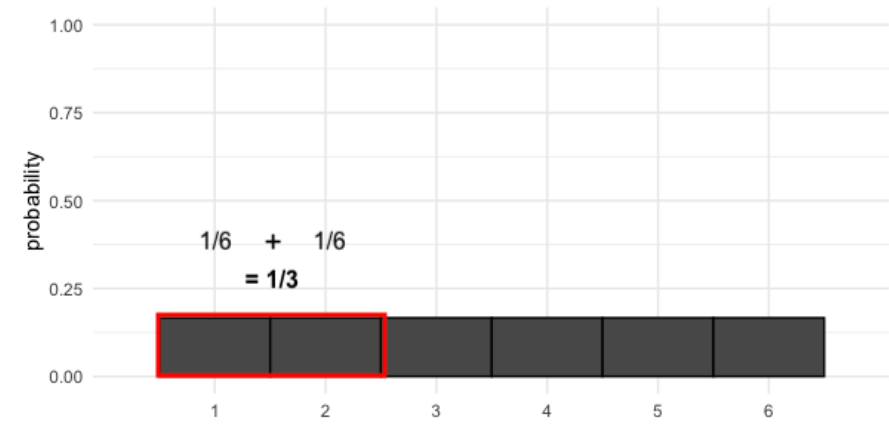
\includegraphics{fig22.png}

\hypertarget{dado-desigual}{%
\subsubsection{Dado desigual}\label{dado-desigual}}

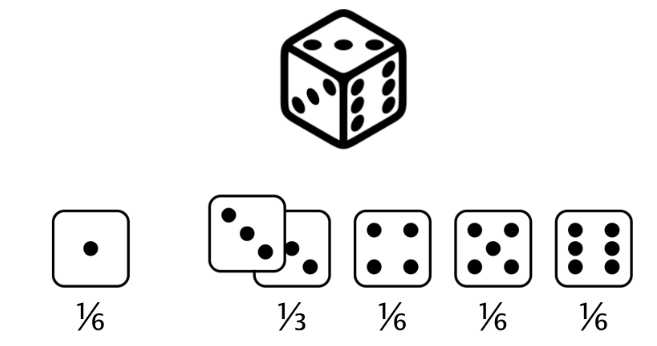
\includegraphics{fig23.png}

Ahora digamos que tenemos un dado donde los dos se convirtieron en tres.
Esto significa que ahora tenemos un 0\% de posibilidades de obtener un 2
y un 33\% de posibilidad de obtener un 3. Matemáticamente esto es

\[
(1\times 1/6) + (1\times 0) + (3\times 1/3) + (4\times 1/6) + (5\times 1/6) + (6\times 1/6) = \fbox{3.67}
\]

ya que es imposible obtener un 2 y un 3 por su nueva probabilidad, un
tercio. Esto nos da un valor esperado que es ligeramente más alto que el
dado justo.

\hypertarget{visualizaciuxf3n-de-probabilidades-desiguales}{%
\subsection{Visualización de Probabilidades
desiguales}\label{visualizaciuxf3n-de-probabilidades-desiguales}}

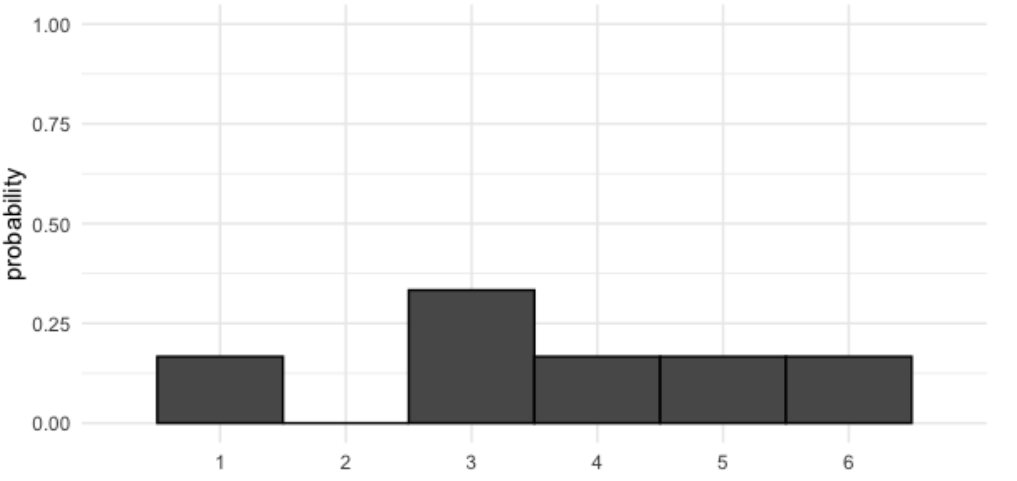
\includegraphics{fig24.png}

Cuando visualizamos estas nuevas probabilidades, las barras ya no son
pares. Con este dado, ¿cuál es la probabilidad de obtener algo menor o
igual a 2?, es decir

\[
P(dado desigual) \leq 2 = ? 
\]

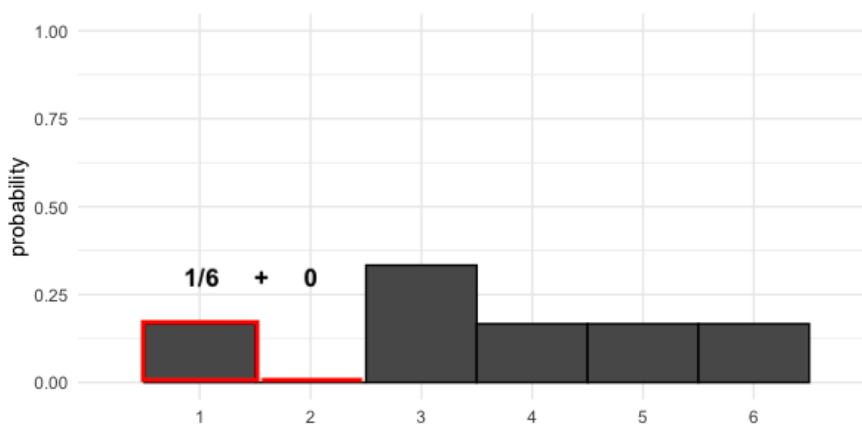
\includegraphics{fig25.png}

Hay un sexto de probabilidad de obtener 1 y cero probabilidad de obtener
2, que suma un sexto, tal como puede ver en la figura previa.

Las distribuciones de probabilidad que ha visto hasta ahora son
discretas, ya que representan situaciones con resultados discretos.
Recuerde del capítulo anterior que las variables discretas pueden
considerarse como variables contables o contadas. En el caso de un dado,
estamos contando puntos, por lo que no podemos sacar 1.5 o 4.3.

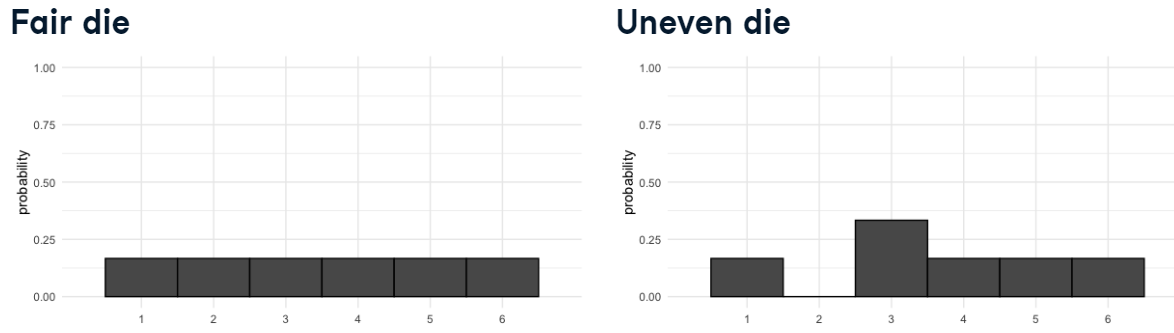
\includegraphics{fig26.png}

\hypertarget{distribuciuxf3n-uniforme}{%
\section{Distribución Uniforme}\label{distribuciuxf3n-uniforme}}

Cuando todos los resultados tienen la misma probabilidad, como un dado
justo, se trata de una distribución especial denominada
\texttt{distribución\ uniforme\ discreta.}

\hypertarget{muestreo-a-partir-de-distribuciones-discretas}{%
\section{Muestreo a partir de distribuciones
discretas}\label{muestreo-a-partir-de-distribuciones-discretas}}

Al igual que tomamos muestras de nombres de una caja, podemos hacer lo
mismo con distribuciones de probabilidad como las que hemos visto. Aquí
hay un marco de datos llamado dado que representa un dado justo y su
valor esperado es 3.5.

\begin{Shaded}
\begin{Highlighting}[]
\NormalTok{dado }\OtherTok{\textless{}{-}} \FunctionTok{data.frame}\NormalTok{(}\AttributeTok{n =} \FunctionTok{c}\NormalTok{(}\DecValTok{1}\NormalTok{, }\DecValTok{2}\NormalTok{, }\DecValTok{3}\NormalTok{, }\DecValTok{4}\NormalTok{, }\DecValTok{5}\NormalTok{, }\DecValTok{6}\NormalTok{))}

\FunctionTok{mean}\NormalTok{(dado}\SpecialCharTok{$}\NormalTok{n)}
\end{Highlighting}
\end{Shaded}

\begin{verbatim}
[1] 3.5
\end{verbatim}

Tomaremos muestras de él 10 veces para simular 10 rollos. Tenga en
cuenta que muestreamos con reemplazo para que estemos muestreando de la
misma distribución cada vez.

\begin{Shaded}
\begin{Highlighting}[]
\FunctionTok{set.seed}\NormalTok{(}\DecValTok{4}\NormalTok{)}
\NormalTok{rolls\_10 }\OtherTok{\textless{}{-}}\NormalTok{ dado }\SpecialCharTok{\%\textgreater{}\%} 
  \FunctionTok{sample\_n}\NormalTok{(}\DecValTok{10}\NormalTok{, }\AttributeTok{replace =} \ConstantTok{TRUE}\NormalTok{)}
\NormalTok{rolls\_10}
\end{Highlighting}
\end{Shaded}

\begin{verbatim}
   n
1  3
2  3
3  3
4  4
5  3
6  6
7  5
8  2
9  3
10 6
\end{verbatim}

\hypertarget{visualizaciuxf3n-de-la-muestra}{%
\subsection{Visualización de la
muestra}\label{visualizaciuxf3n-de-la-muestra}}

Podemos visualizar los resultados de los diez lanzamientos usando un
histograma, estableciendo el número de contenedores en 6 ya que hay 6
resultados posibles.

\begin{Shaded}
\begin{Highlighting}[]
\FunctionTok{library}\NormalTok{(ggplot2)}
\FunctionTok{ggplot}\NormalTok{(rolls\_10, }\FunctionTok{aes}\NormalTok{(n)) }\SpecialCharTok{+} 
  \FunctionTok{geom\_histogram}\NormalTok{(}\AttributeTok{bins =} \DecValTok{6}\NormalTok{)}
\end{Highlighting}
\end{Shaded}

\begin{figure}[H]

{\centering 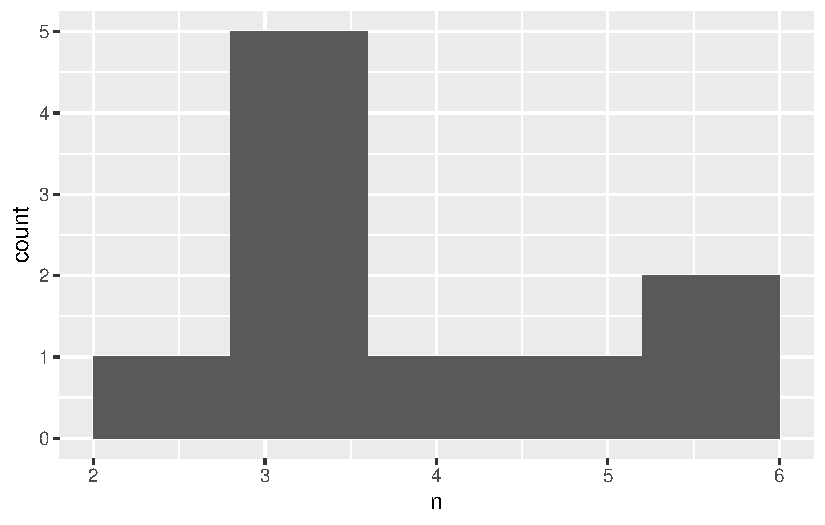
\includegraphics{summary_files/figure-pdf/unnamed-chunk-10-1.pdf}

}

\end{figure}

\hypertarget{distribuciuxf3n-muestral-vs-distribuciuxf3n-teuxf3rica}{%
\section{Distribución muestral vs distribución
teórica}\label{distribuciuxf3n-muestral-vs-distribuciuxf3n-teuxf3rica}}

Observe que tenemos diferentes números de 1,2,3, etc., ya que la muestra
fue aleatoria, aunque cada tirada teníamos la misma probabilidad de
sacar cada una.

La media de nuestra muestra es de 3.3, que no esta tan cerca del 3.5 que
esperabamos.

\begin{Shaded}
\begin{Highlighting}[]
\FunctionTok{mean}\NormalTok{(rolls\_10}\SpecialCharTok{$}\NormalTok{n)}
\end{Highlighting}
\end{Shaded}

\begin{verbatim}
[1] 3.8
\end{verbatim}

\begin{Shaded}
\begin{Highlighting}[]
\FunctionTok{mean}\NormalTok{(dado}\SpecialCharTok{$}\NormalTok{n)}
\end{Highlighting}
\end{Shaded}

\begin{verbatim}
[1] 3.5
\end{verbatim}

\hypertarget{una-muestra-muxe1s-grande}{%
\subsection{Una muestra más grande}\label{una-muestra-muxe1s-grande}}

Si lanzamos el dado 100 veces, la distribución de las tiradas se ve un
poco más uniforme y la media esta más cerca de 3.5

\begin{Shaded}
\begin{Highlighting}[]
\FunctionTok{set.seed}\NormalTok{(}\DecValTok{1}\NormalTok{)}
\NormalTok{rolls\_100 }\OtherTok{\textless{}{-}}\NormalTok{ dado }\SpecialCharTok{\%\textgreater{}\%} 
  \FunctionTok{sample\_n}\NormalTok{(}\DecValTok{100}\NormalTok{, }\AttributeTok{replace =} \ConstantTok{TRUE}\NormalTok{)}

\FunctionTok{mean}\NormalTok{(rolls\_100}\SpecialCharTok{$}\NormalTok{n)}
\end{Highlighting}
\end{Shaded}

\begin{verbatim}
[1] 3.52
\end{verbatim}

\begin{Shaded}
\begin{Highlighting}[]
\FunctionTok{ggplot}\NormalTok{(rolls\_100, }\FunctionTok{aes}\NormalTok{(n)) }\SpecialCharTok{+} 
  \FunctionTok{geom\_histogram}\NormalTok{(}\AttributeTok{bins =} \DecValTok{6}\NormalTok{)}
\end{Highlighting}
\end{Shaded}

\begin{figure}[H]

{\centering 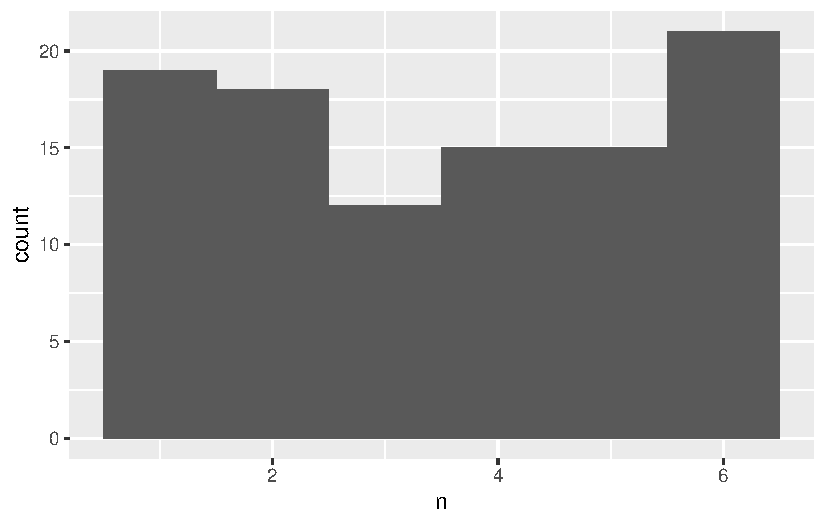
\includegraphics{summary_files/figure-pdf/unnamed-chunk-14-1.pdf}

}

\end{figure}

\hypertarget{ley-de-los-grandes-nuxfameros}{%
\subsection{Ley de los grandes
números}\label{ley-de-los-grandes-nuxfameros}}

Esto se llama la ley de los grandes números, que es la idea de que a
medida que aumenta el tamaño de la muestra, la media de la muestra se
acercará a la ,media teórica.

\hypertarget{ejercicio-7}{%
\section{Ejercicio 7}\label{ejercicio-7}}

En este ejercicio vamos a crear una distribución de probabilidad.

Suponga que un nuevo restaurante abrió hace unos meses y la gerencia del
restaurante quiere optimizar su espacio para sentarse en función del
tamaño de los grupos que vienen con más frecuencia. En una noche, hay 10
grupos de personas esperando para sentarse en el restaurante, pero en
lugar de ser llamados en el orden que llegaron, serán llamados al azar.
Creemos hipoteticamente nuestra data

\begin{Shaded}
\begin{Highlighting}[]
\NormalTok{restaurant\_groups }\OtherTok{\textless{}{-}} \FunctionTok{data.frame}\NormalTok{(}\AttributeTok{group\_id =} \FunctionTok{c}\NormalTok{(}\StringTok{"A"}\NormalTok{, }\StringTok{"B"}\NormalTok{, }\StringTok{"C"}\NormalTok{, }\StringTok{"D"}\NormalTok{, }\StringTok{"E"}\NormalTok{, }\StringTok{"F"}\NormalTok{, }\StringTok{"G"}\NormalTok{, }\StringTok{"H"}\NormalTok{, }\StringTok{"I"}\NormalTok{, }\StringTok{"J"}\NormalTok{), }\AttributeTok{group\_size =} \FunctionTok{c}\NormalTok{(}\DecValTok{2}\NormalTok{, }\DecValTok{4}\NormalTok{, }\DecValTok{6}\NormalTok{, }\DecValTok{2}\NormalTok{, }\DecValTok{2}\NormalTok{, }\DecValTok{2}\NormalTok{, }\DecValTok{3}\NormalTok{, }\DecValTok{2}\NormalTok{, }\DecValTok{4}\NormalTok{, }\DecValTok{2}\NormalTok{))}
\end{Highlighting}
\end{Shaded}

En este ejercicio, investigará la probabilidad de que grupos de
diferentes tamaños de cada uno de los diez grupos están contenidos en el
marco de datos \texttt{restaurant\_groups}.

Primero cree un histograma de la columna \texttt{group\_size} de
\texttt{restaurant\_groups}, estableciendo el número de contenedores en
5.

\begin{Shaded}
\begin{Highlighting}[]
\FunctionTok{ggplot}\NormalTok{(restaurant\_groups, }\FunctionTok{aes}\NormalTok{(group\_size)) }\SpecialCharTok{+}
  \FunctionTok{geom\_histogram}\NormalTok{(}\AttributeTok{bins =} \DecValTok{5}\NormalTok{)}
\end{Highlighting}
\end{Shaded}

\begin{figure}[H]

{\centering 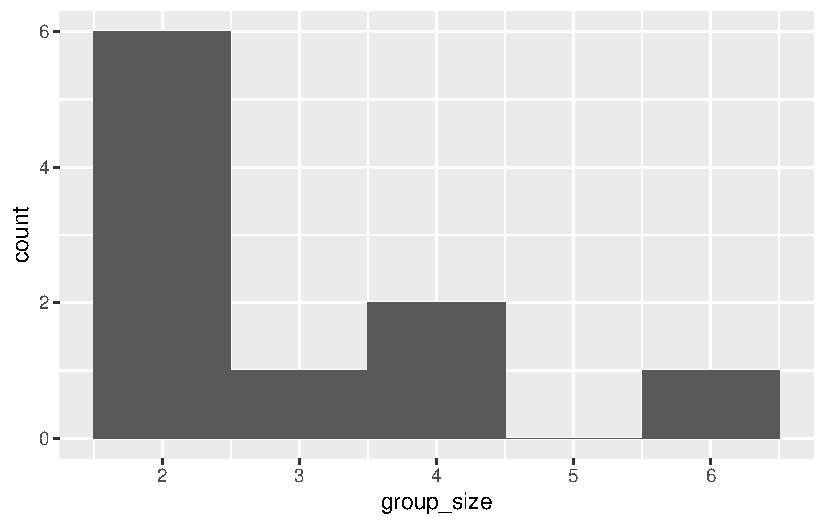
\includegraphics{summary_files/figure-pdf/unnamed-chunk-16-1.pdf}

}

\end{figure}

Ahora, cuente el número de cada uno de los \texttt{group\_size} en
\texttt{restaurant\_groups}, luego agregue una columna llamada
\texttt{probability} que contiene la probabilidad de seleccionar
aleatoriamente un grupo de cada tamaño. Almacene esto en un nuevo marco
de datos llamado \texttt{size\_distribution}.

\begin{Shaded}
\begin{Highlighting}[]
\NormalTok{size\_distribution }\OtherTok{\textless{}{-}}\NormalTok{restaurant\_groups }\SpecialCharTok{\%\textgreater{}\%}
  \CommentTok{\# contamos el número de cada tamaño de grupo}
  \FunctionTok{count}\NormalTok{(group\_size) }\SpecialCharTok{\%\textgreater{}\%}
  \CommentTok{\# Calculamos las probabilidades}
  \FunctionTok{mutate}\NormalTok{(}\AttributeTok{probability =}\NormalTok{ n }\SpecialCharTok{/} \FunctionTok{sum}\NormalTok{(n))}

\NormalTok{size\_distribution}
\end{Highlighting}
\end{Shaded}

\begin{verbatim}
  group_size n probability
1          2 6         0.6
2          3 1         0.1
3          4 2         0.2
4          6 1         0.1
\end{verbatim}

Ahora, dado que ya tenemos las probabilidades, estamos listos para
calcular el valor esperado de \texttt{size\_distribution}, que
representa el tamaño esperado del grupo.

\begin{Shaded}
\begin{Highlighting}[]
\NormalTok{expected\_val }\OtherTok{\textless{}{-}} \FunctionTok{sum}\NormalTok{(size\_distribution}\SpecialCharTok{$}\NormalTok{group\_size }\SpecialCharTok{*}\NormalTok{ size\_distribution}\SpecialCharTok{$}\NormalTok{probability)}
\NormalTok{expected\_val}
\end{Highlighting}
\end{Shaded}

\begin{verbatim}
[1] 2.9
\end{verbatim}

Por último, calculamos la probabilidad de elegir aleatoriamente un grupo
de 4 o más personas filtrando y resumiendo.

\begin{Shaded}
\begin{Highlighting}[]
\NormalTok{size\_distribution }\SpecialCharTok{\%\textgreater{}\%}
  \CommentTok{\# Filtramos para grupos de 4 o mas }
  \FunctionTok{filter}\NormalTok{(group\_size }\SpecialCharTok{\textgreater{}=} \DecValTok{4}\NormalTok{) }\SpecialCharTok{\%\textgreater{}\%}
  \CommentTok{\# Calculamos la prob\_4\_o\_mas tomando la suma de probabilidades}
  \FunctionTok{summarize}\NormalTok{(}\AttributeTok{prob\_4\_or\_more =} \FunctionTok{sum}\NormalTok{(probability))}
\end{Highlighting}
\end{Shaded}

\begin{verbatim}
  prob_4_or_more
1            0.3
\end{verbatim}

\hypertarget{indentificaciuxf3n-de-distribuciones}{%
\subsection{Indentificación de
distribuciones}\label{indentificaciuxf3n-de-distribuciones}}

¿Qué muestra es más probable que se haya tomado de una distribución
uniforme?

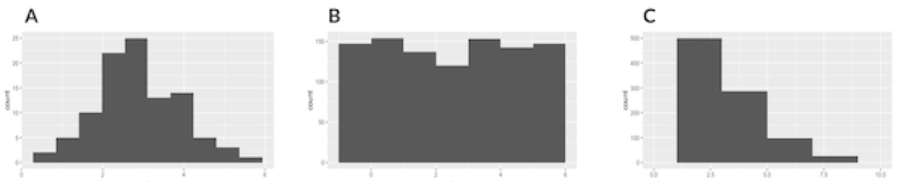
\includegraphics{fig27.png}

\textbf{Respuesta: Opción B}

\hypertarget{distribuciones-continuas}{%
\section{Distribuciones Continuas}\label{distribuciones-continuas}}

Podemos usar distribuciones discretas para modelar situaciones que
involucran variables discretas o contables, pero ¿cómo podemos modelas
variables continuas?

Comencemos con un ejemplo.

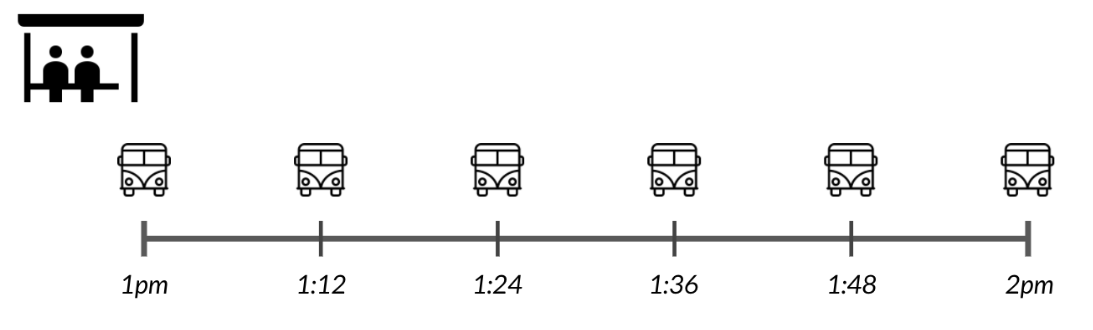
\includegraphics{fig28.png}

El autobús de la ciudad llega cada doce minutos, por lo que si te
presentas a una hora aleatoria, que podrías esperar desde 0 minutos si
llegas justo cuando llega el autobús, hasta 12 minutos si llegas cuando
el autobus sale.

\hypertarget{distribuciuxf3n-uniforme-continua}{%
\subsection{Distribución uniforme
continua}\label{distribuciuxf3n-uniforme-continua}}

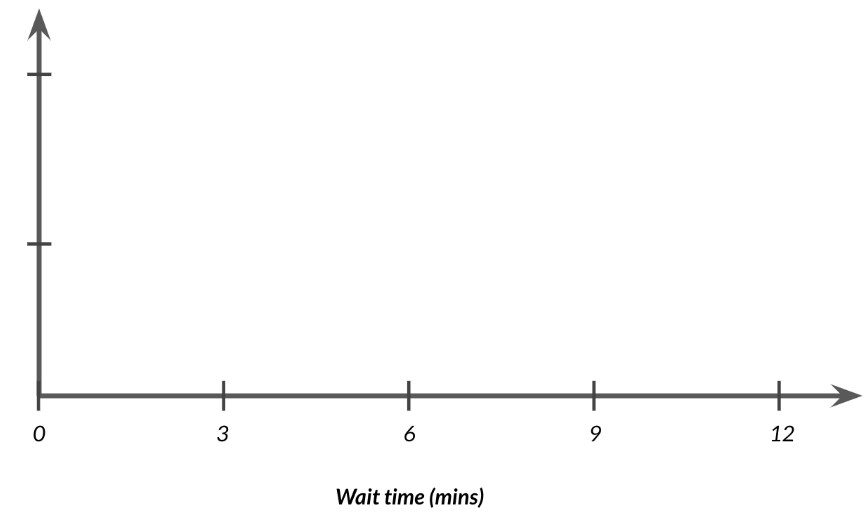
\includegraphics{fig29.png}

Modelemos este escenario con una distribución de probabilidad. Hay una
cantidad infinita de minutos que podríamos esperar, ya que podríamos
esperar 1 minuto, 1.5 minutos, 1.53 minutos, etc., por lo que no podemos
crear bloques individuales como la hariamos con una variable discreta.

En cambio, usaremos una línea continua para representar la probabilidad.
La linea es plana ya que existe la misma probabilidad de esperar
cualquier tiempo de 0 a 12 minutos. Esto se llama la
\texttt{distribución\ uniforme\ continua.}

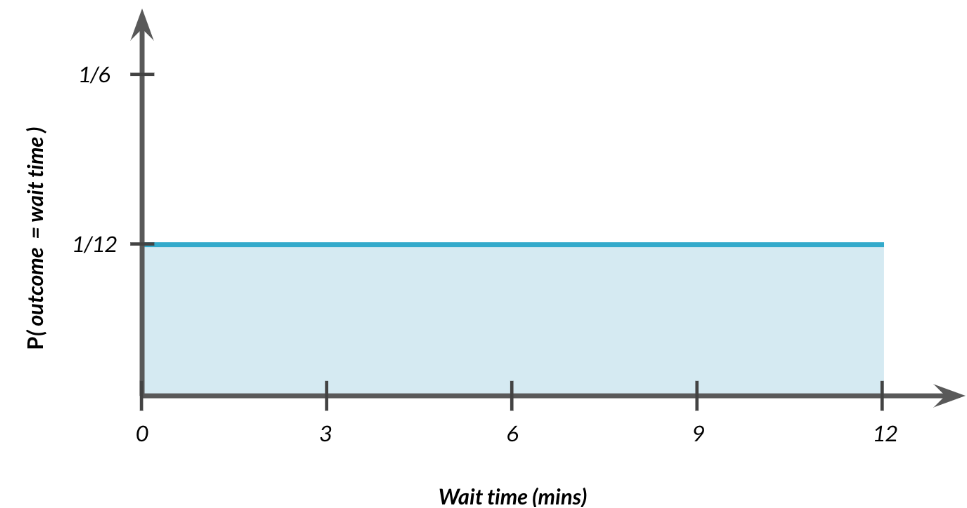
\includegraphics{fig30.png}

Ahora que tenemos nuestra distribución, averiguemos cual es la
probabilidad de que esperemos entre 4 y 7 minutos. Al igual que con las
distribuciones discretas , podemos tomar el área de 4 a 7 para calcular
la probabilidad.

\[
P(4\leq \mbox{tiempo de espera} \leq 7) = ?
\]

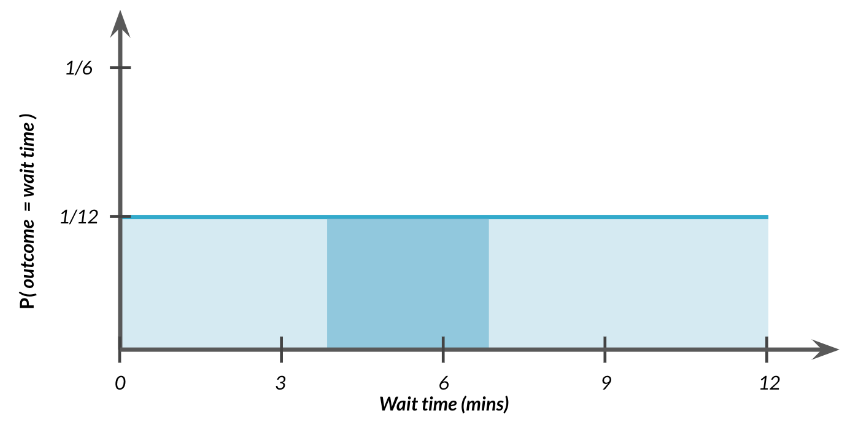
\includegraphics{fig31.png}

Al igual que con las distribuciones discretas, podemos tomar el área de
4 a 7 para calcular la probabilidad.

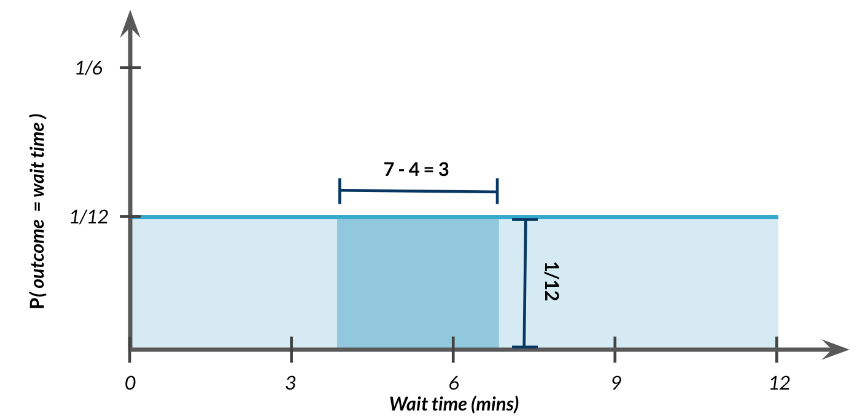
\includegraphics{fig32.png}

El ancho de este rectángulo es 7 menos 4 que es 3. La altura es 1/12,
entonces

\[
P(4\leq \mbox{tiempo espera}\leq 7) = 3\times \frac{1}{12} = \frac{1}{4} = \fbox{25\%}
\]

\hypertarget{distribuciuxf3n-uniforme-en-r}{%
\subsection{Distribución Uniforme en
R}\label{distribuciuxf3n-uniforme-en-r}}

Usemos la distribución uniforme en R para calcular la probabilidad de
esperar 7 minutos o menos. Pasaremos 7 a \texttt{punif} función que nos
ayuda a calcular la probabilidad uniforme en R. Veamos:

\begin{Shaded}
\begin{Highlighting}[]
\FunctionTok{punif}\NormalTok{(}\DecValTok{7}\NormalTok{, }\AttributeTok{min =} \DecValTok{0}\NormalTok{, }\AttributeTok{max =} \DecValTok{12}\NormalTok{)}
\end{Highlighting}
\end{Shaded}

\begin{verbatim}
[1] 0.5833333
\end{verbatim}

Por tanto, la probabilidad de esperar menos de 7 minutos es del
\(\fbox{58\%}\).

\hypertarget{cola-inferior}{%
\subsection{Cola Inferior}\label{cola-inferior}}

Si queremos la probabilidad de esperar más de 7 minutos,

\[P(\mbox{tiempo de espera} \geq 7) = ?\]establezca el argumento de cola
de punto inferior en FALSO.

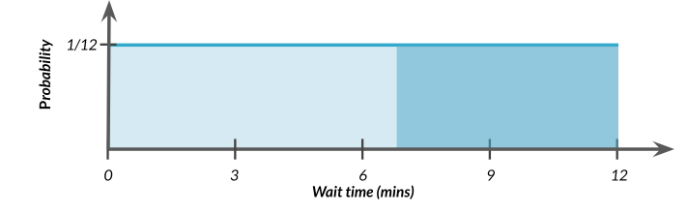
\includegraphics{fig33.png}

En R esto es:

\begin{Shaded}
\begin{Highlighting}[]
\FunctionTok{punif}\NormalTok{(}\DecValTok{7}\NormalTok{, }\AttributeTok{min =} \DecValTok{0}\NormalTok{, }\AttributeTok{max =} \DecValTok{12}\NormalTok{, }\AttributeTok{lower.tail =} \ConstantTok{FALSE}\NormalTok{)}
\end{Highlighting}
\end{Shaded}

\begin{verbatim}
[1] 0.4166667
\end{verbatim}

Pero, ¿cómo calculamos la probabilidad de esperar de 4 a 7 minutos
usando R?

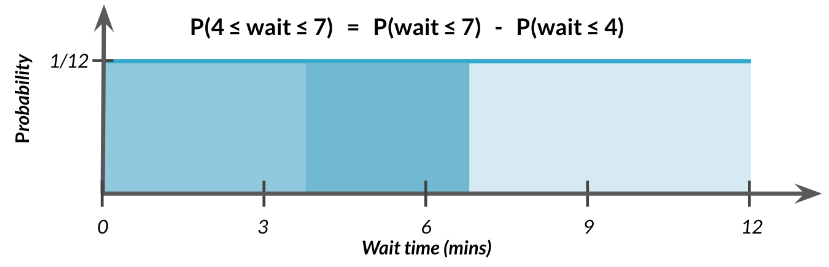
\includegraphics{fig34.png}

Podemos empezar con la probabilidad de esperar menos de 7 minutos, luego
reste la probabilidad de esperar menos de 4 minutos, tal como puede
apreciar en la figura. En R esto es:

\begin{Shaded}
\begin{Highlighting}[]
\FunctionTok{punif}\NormalTok{(}\DecValTok{7}\NormalTok{, }\AttributeTok{min =} \DecValTok{0}\NormalTok{, }\AttributeTok{max =} \DecValTok{12}\NormalTok{) }\SpecialCharTok{{-}} \FunctionTok{punif}\NormalTok{(}\DecValTok{4}\NormalTok{, }\AttributeTok{min =} \DecValTok{0}\NormalTok{, }\AttributeTok{max =} \DecValTok{12}\NormalTok{)}
\end{Highlighting}
\end{Shaded}

\begin{verbatim}
[1] 0.25
\end{verbatim}

Para calcular la probabilidad de esperar entre 0 y 12 minutos

\[
P(0\leq \mbox{tiempo de espera}\leq 12) = ?
\]

Graficamente esto es

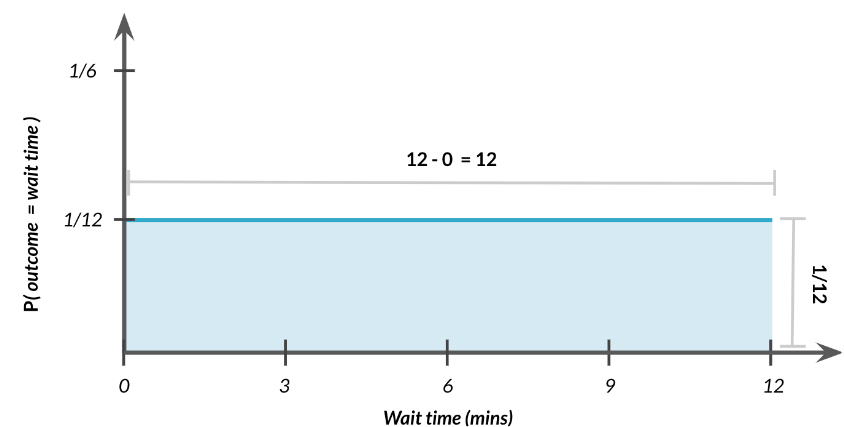
\includegraphics{fig35.png}

Por tanto, no es mas que multiplicar 12 por 1/2, es decir:

\[
P(0\leq \mbox{tiempo de espera}\leq 12) = 12\times \frac{1}{12} = \fbox{1}
\]

Esto tiene sentido ya que estamos eguros que esperaremos entre 0 y 12
minutos.

\hypertarget{otras-distribuciones-continuas}{%
\subsection{Otras Distribuciones
Continuas}\label{otras-distribuciones-continuas}}

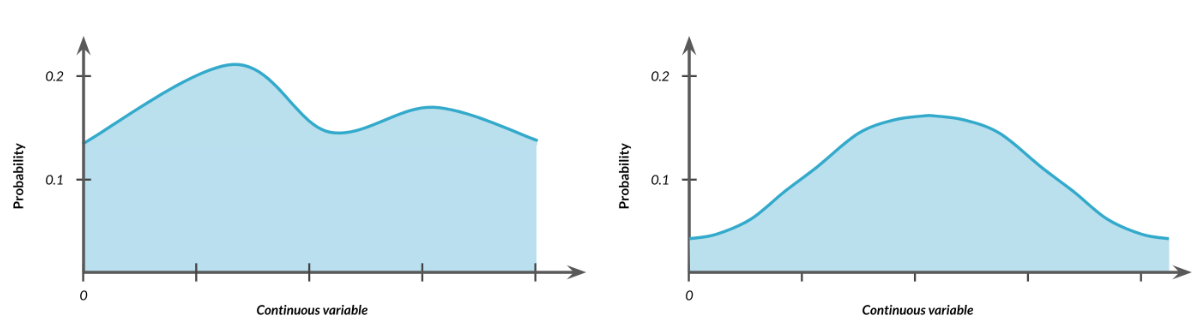
\includegraphics{fig36.png}

Las distribuciones continuas pueden tomar formas distintas a las
uniformes donde algunos valores tienen una probabilidad mayor que otros.
No importa la forma de la distribución, el área debajo de ella siempre
debe de ser igual a 1.

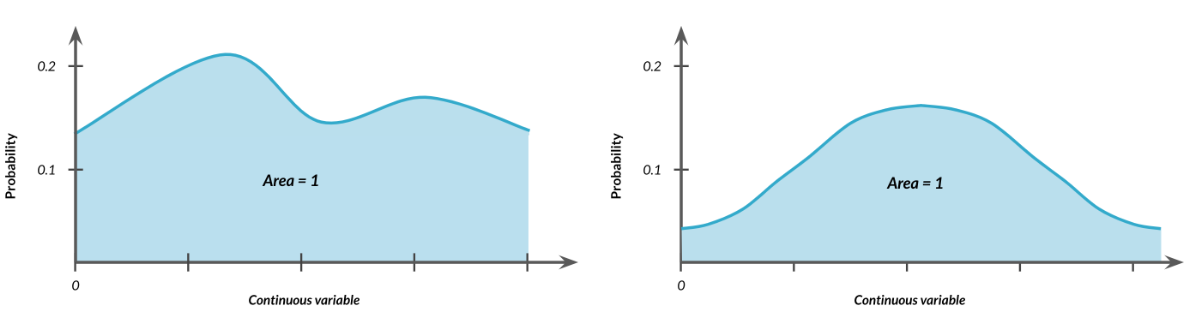
\includegraphics{fig37.png}

Esto también se aplicará a otras distribuciones que aprenderemos más
adelante en este curso, como la distribución normal o distribución de
Poisson, que se puede usar para modelar muchas situaciones de la vida
real.

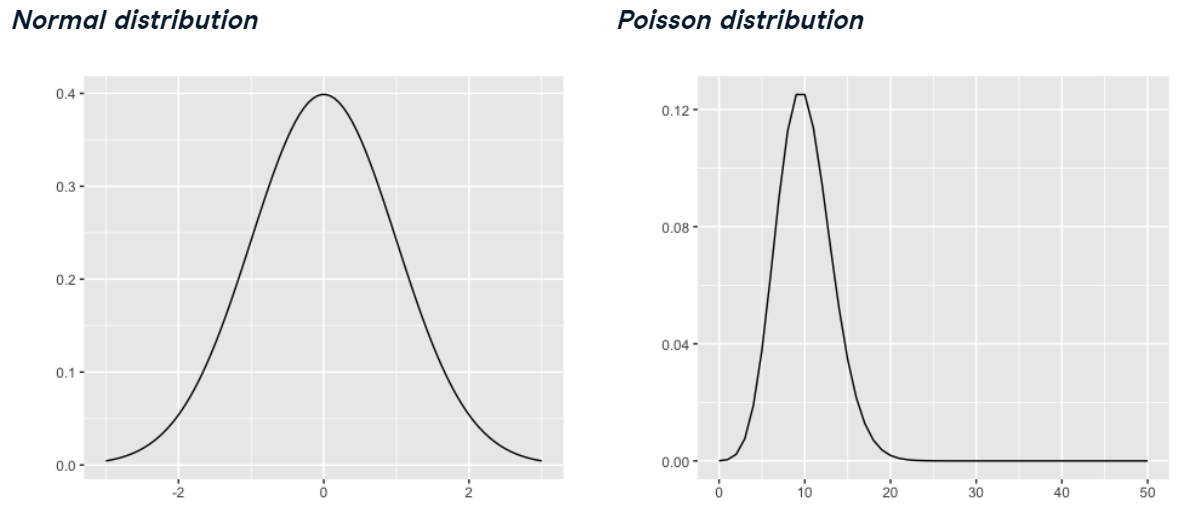
\includegraphics{fig38.png}

\hypertarget{ejercicio-8}{%
\section{Ejercicio 8}\label{ejercicio-8}}

En este punto, ha aprendido acerca de las dos variantes diferentes de la
distribución uniforme: la distribución uniforme discreta y la
distribución uniforme continua. en este ejercicio, decidirá qué
situaciones siguen qué distribución.

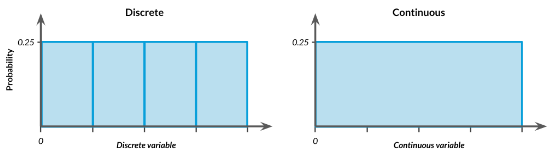
\includegraphics{fig39.png}

Asignaremos cada situación a la distribución de probabilidad con la que
se modelaría mejor.

\begin{longtable}[]{@{}
  >{\raggedright\arraybackslash}p{(\columnwidth - 4\tabcolsep) * \real{0.2917}}
  >{\raggedright\arraybackslash}p{(\columnwidth - 4\tabcolsep) * \real{0.5000}}
  >{\raggedright\arraybackslash}p{(\columnwidth - 4\tabcolsep) * \real{0.2083}}@{}}
\toprule\noalign{}
\begin{minipage}[b]{\linewidth}\raggedright
Uniforme discreto
\end{minipage} & \begin{minipage}[b]{\linewidth}\raggedright
Uniforme continuo
\end{minipage} & \begin{minipage}[b]{\linewidth}\raggedright
Otro
\end{minipage} \\
\midrule\noalign{}
\endhead
\bottomrule\noalign{}
\endlastfoot
El número de boleto de un ganador de la rifa, suponiendo que haya un
boleto para cada número del 1 al 100. & La hora del día en que nacerá un
bebé. & La altura de una persona al azar. \\
El resultado de lanzar un dado de 4 caras. & El tiempo que tendrás que
esperar para que un géiser entre en erupción si te presentas en un
momento aleatorio, sabiendo que el géiser entra en erupción exactamente
cada diez minutos. & \\
\end{longtable}

\hypertarget{ejercicio-9}{%
\section{Ejercicio 9}\label{ejercicio-9}}

El software de ventas utilizado en su empresa está configurado para
realizar copias de seguridad automaáicamente, pero nadie sabe
exactamente a qué hora se realizan las copias de seguridad. Sin embargo,
se sabe que las copias de seguridad se realizan exactamente cada 30
minutos. Amir regresa de las reuniones de ventas en momentos aleatorios
para actualizar los datos del cliente con el que acaba de reunirse.
Quiere saber cuánto tiempo tendrá que esperar para que realice una copia
de seguridad de sus datos recién ingresados. Usando nuestro nuevo
conocimiento de distribuciones uniformes continuas para modelar esta
situación y responder las preguntas de Amir.

\begin{itemize}
\item
  Primero, para modelar cuánto tiempo esperará Amir por una copia de
  seguridad utilizando una distribución uniforme continua, guarde su
  tiempo de espera más bajo posible como \texttt{min} y su tiempo de
  espera más alto posible como \texttt{max}. Recuerde que las copias de
  seguridad se realizan cada 30 minutos.

\begin{Shaded}
\begin{Highlighting}[]
\CommentTok{\# Tiempos de espera mínimos y máximos para la copia de seguridad que se realiza cada 30 minutos}
\NormalTok{min }\OtherTok{\textless{}{-}} \DecValTok{0}
\NormalTok{max }\OtherTok{\textless{}{-}} \DecValTok{30}
\end{Highlighting}
\end{Shaded}
\item
  Calculemos la probabilidad de que Amir tenga que esperar menos menos
  de 5 minutos y guárdala en una nueva variable llamada
  \texttt{prob\_less\_than\_5}.

\begin{Shaded}
\begin{Highlighting}[]
\NormalTok{prob\_less\_than\_5 }\OtherTok{\textless{}{-}} \FunctionTok{punif}\NormalTok{(}\DecValTok{5}\NormalTok{, }\AttributeTok{min =}\NormalTok{ min, }\AttributeTok{max =}\NormalTok{ max)}
\NormalTok{prob\_less\_than\_5}
\end{Highlighting}
\end{Shaded}

\begin{verbatim}
[1] 0.1666667
\end{verbatim}
\item
  Ahora, calculemos la probabilidad de que Amir tenga que esperar más de
  5 minutos y guárdala en una variable llamada
  \texttt{prob\_greater\_than\_5}.

\begin{Shaded}
\begin{Highlighting}[]
\NormalTok{prob\_greater\_than\_5 }\OtherTok{\textless{}{-}} \FunctionTok{punif}\NormalTok{(}\DecValTok{30}\NormalTok{, }\AttributeTok{min =}\NormalTok{ min, }\AttributeTok{max=}\NormalTok{ max)}\SpecialCharTok{{-}} \FunctionTok{punif}\NormalTok{(}\DecValTok{5}\NormalTok{, }\AttributeTok{min =}\NormalTok{ min, }\AttributeTok{max =}\NormalTok{ max)}
\NormalTok{prob\_greater\_than\_5}
\end{Highlighting}
\end{Shaded}

\begin{verbatim}
[1] 0.8333333
\end{verbatim}
\item
  Por último calcule la probabilidad de que Amir tenga que esperar entre
  10 y 20 minutos, y guárdala en una nueva variable llamada
  \texttt{prob\_between\_10\_end\_20}.

\begin{Shaded}
\begin{Highlighting}[]
\NormalTok{prob\_between\_10\_and\_20 }\OtherTok{\textless{}{-}} \FunctionTok{punif}\NormalTok{(}\DecValTok{20}\NormalTok{, }\AttributeTok{min =}\NormalTok{ min, }\AttributeTok{max =}\NormalTok{ max) }\SpecialCharTok{{-}} \FunctionTok{punif}\NormalTok{(}\DecValTok{10}\NormalTok{, }\AttributeTok{min =}\NormalTok{ min, }\AttributeTok{max =}\NormalTok{ max)}
\NormalTok{prob\_between\_10\_and\_20}
\end{Highlighting}
\end{Shaded}

\begin{verbatim}
[1] 0.3333333
\end{verbatim}
\end{itemize}

\hypertarget{ejercicio-10}{%
\section{Ejercicio 10}\label{ejercicio-10}}

Para darle a Amir una mejor idea de cuánto tiempo tendrá que esperar,
simularemos la esperá de Amir 1000 veces y creará un histograma para
mostrarle lo que debe esperar. Recuerde del último ejercicio que su
tiempo de espera mínimo es de 0 minutos y su tiempo de espera máximo es
de 30 minutos.

Creemos un marcos de datos llamado \texttt{wait\_times} y establezcamos
un valor semilla de 334.

\begin{Shaded}
\begin{Highlighting}[]
\FunctionTok{set.seed}\NormalTok{(}\DecValTok{334}\NormalTok{)}
\NormalTok{wait\_times }\OtherTok{\textless{}{-}} \FunctionTok{data.frame}\NormalTok{(}\AttributeTok{simulation\_nb =} \FunctionTok{c}\NormalTok{(}\FunctionTok{seq}\NormalTok{(}\DecValTok{1}\SpecialCharTok{:}\DecValTok{1000}\NormalTok{)))}
\FunctionTok{head}\NormalTok{(wait\_times)}
\end{Highlighting}
\end{Shaded}

\begin{verbatim}
  simulation_nb
1             1
2             2
3             3
4             4
5             5
6             6
\end{verbatim}

Ahora, generamos 1000 tiempos de espera a partir de la distribución
uniforme continua que modela el tiempo de espera de Amir. Agregue esto
como una nueva columna llamada \texttt{time} en el marco de datos
\texttt{wait\_times}.

\begin{Shaded}
\begin{Highlighting}[]
\NormalTok{wait\_times\_1000 }\OtherTok{\textless{}{-}}\NormalTok{ wait\_times }\SpecialCharTok{\%\textgreater{}\%}
  \FunctionTok{mutate}\NormalTok{(}\AttributeTok{time =} \FunctionTok{runif}\NormalTok{(}\DecValTok{1000}\NormalTok{, }\AttributeTok{min =} \DecValTok{0}\NormalTok{, }\AttributeTok{max =} \DecValTok{30}\NormalTok{))}
\end{Highlighting}
\end{Shaded}

Luego, creamos el histograma de los tiempos de espera simulados con 30
contenedores.

\begin{Shaded}
\begin{Highlighting}[]
\NormalTok{wait\_times\_1000 }\SpecialCharTok{\%\textgreater{}\%}
  \FunctionTok{mutate}\NormalTok{(}\AttributeTok{time =} \FunctionTok{runif}\NormalTok{(}\DecValTok{1000}\NormalTok{, }\AttributeTok{min =} \DecValTok{0}\NormalTok{, }\AttributeTok{max =} \DecValTok{30}\NormalTok{)) }\SpecialCharTok{\%\textgreater{}\%}
  \FunctionTok{ggplot}\NormalTok{(}\FunctionTok{aes}\NormalTok{(time)) }\SpecialCharTok{+}
  \FunctionTok{geom\_histogram}\NormalTok{(}\AttributeTok{bins =} \DecValTok{30}\NormalTok{)}
\end{Highlighting}
\end{Shaded}

\begin{figure}[H]

{\centering 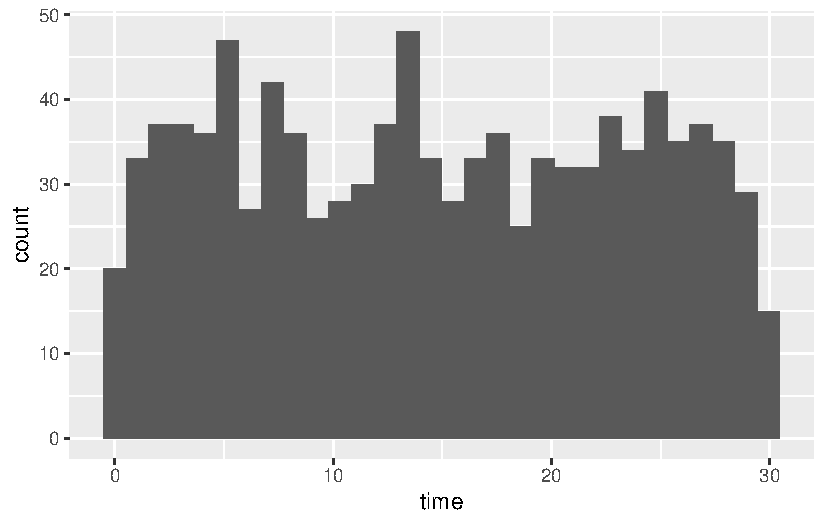
\includegraphics{summary_files/figure-pdf/unnamed-chunk-29-1.pdf}

}

\end{figure}

Excelente simulación! A menos que Amir descubra exactamente a qué hora
ocurre cada copia de seguridad, no podrá programar la entrada de datos
para que se haga una copia de seguridad antes, pero parece que esperará
unos 15 minutos en promedio.

\hypertarget{distribuciuxf3n-binomial}{%
\section{Distribución Binomial}\label{distribuciuxf3n-binomial}}

Es hora de ampliar aún más su caja de herramientas de distribuciones. En
este sección, aprenderá sobre la distribución bonomial.

\hypertarget{lanzamiento-de-monedas}{%
\subsection{Lanzamiento de monedas}\label{lanzamiento-de-monedas}}

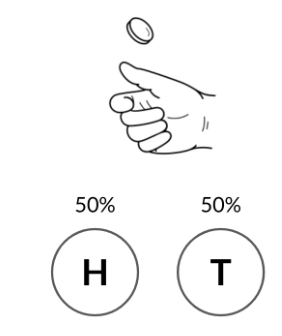
\includegraphics{fig40.png}

Comenzaremos lanzando una moneda, que tiene dos resultados posibles,
cara o cruz, cada uno con una probabilidad del 50\%.

\hypertarget{resultados-binarios}{%
\subsection{Resultados Binarios}\label{resultados-binarios}}

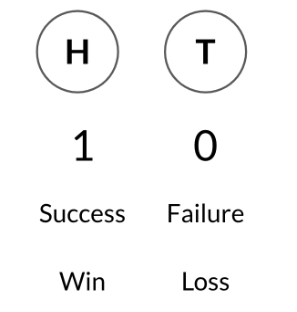
\includegraphics{fig41.png}

Este es un ejemplo de un resultado binario, o un resultado con dos
valores prosibles. También podríamos respresentar estos resultados como
un \texttt{1} y un \texttt{0}, un éxito o un fracaso, y una victoria o
una derrota.

En \texttt{R}, podemos simular esto usando la función \texttt{rbinom},
que toma en cuenta la cantidad de intentos o veces que queremos lanzar,
la cantidad de monedas que queremos lanzar y la probabilidad de cara o
éxito. Esto devolverá un 1 que contaremos como cara o un 0 que
contaremos como cruz. Podemos usar

\begin{Shaded}
\begin{Highlighting}[]
\FunctionTok{rbinom}\NormalTok{(}\DecValTok{1}\NormalTok{, }\DecValTok{1}\NormalTok{, }\FloatTok{0.5}\NormalTok{)}
\end{Highlighting}
\end{Shaded}

\begin{verbatim}
[1] 1
\end{verbatim}

Para realizar ocho lanzamientos de moneda, podemos cambiar el primer
argumento un 8, lo que nos dará ocho lanzamientos de una moneda con un
50\% de prosibilidades de cara. Esto nos da un conjunto de 8 unos y
ceros.

\begin{Shaded}
\begin{Highlighting}[]
\FunctionTok{rbinom}\NormalTok{(}\DecValTok{8}\NormalTok{, }\DecValTok{1}\NormalTok{, }\FloatTok{0.5}\NormalTok{)}
\end{Highlighting}
\end{Shaded}

\begin{verbatim}
[1] 0 0 0 0 0 0 0 1
\end{verbatim}

\hypertarget{muchas-volteretas-una-vez}{%
\subsection{Muchas volteretas una vez}\label{muchas-volteretas-una-vez}}

Si intercambiamos los dos primeros argumentos, simulamos un lanzamiento
de 8 monedas. Esto nos da un número, que es el número total de caras o
éxitos.

\begin{Shaded}
\begin{Highlighting}[]
\FunctionTok{rbinom}\NormalTok{(}\DecValTok{1}\NormalTok{, }\DecValTok{8}\NormalTok{, }\FloatTok{0.5}\NormalTok{)}
\end{Highlighting}
\end{Shaded}

\begin{verbatim}
[1] 4
\end{verbatim}

\hypertarget{muchas-volteretas-muchas-veces}{%
\subsection{Muchas volteretas muchas
veces}\label{muchas-volteretas-muchas-veces}}

De manera similar, podemos pasar 10 y 3 a rbinom para simular 10
lanzamientos de 3 monedas. Esto devuelve 10 números, cada uno de los
cuales representa el número total de caras de cada conjunto de
lanzamientos.

\begin{Shaded}
\begin{Highlighting}[]
\FunctionTok{rbinom}\NormalTok{(}\DecValTok{10}\NormalTok{, }\DecValTok{3}\NormalTok{, }\FloatTok{0.5}\NormalTok{)}
\end{Highlighting}
\end{Shaded}

\begin{verbatim}
 [1] 0 0 2 2 2 1 3 1 1 1
\end{verbatim}

\hypertarget{otras-probabilidades}{%
\subsection{Otras probabilidades}\label{otras-probabilidades}}

También podríamos tener una moneda que sea más pesada en un lado que en
el otro, por lo que la probabilidad de obtener cara es solo del 25\%.

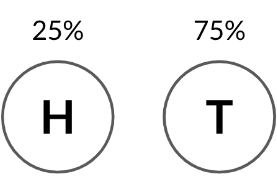
\includegraphics{fig42.png}

Para simular lanzamientos con esta moneda, ajustaremos el tercer
argumento de rbinom a 0.25. El resultado tiene números más bajos, ya que
no es tan probable obtener varias caras con la nueva moneda.

\begin{Shaded}
\begin{Highlighting}[]
\FunctionTok{rbinom}\NormalTok{(}\DecValTok{10}\NormalTok{, }\DecValTok{3}\NormalTok{, }\FloatTok{0.25}\NormalTok{)}
\end{Highlighting}
\end{Shaded}

\begin{verbatim}
 [1] 1 1 0 0 0 0 1 1 1 2
\end{verbatim}

\hypertarget{distribuciuxf3n-binomial-1}{%
\section{Distribución Binomial}\label{distribuciuxf3n-binomial-1}}

La distribución binomial describle la probabilidad del número de éxitos
en una secuencia de ensayos independientes. En otras palabras, puede
decirnos la probabilidad de obtener cierto número de caras en una
secuencia de lanzamientos de monedas. Tenga en cuenta que esta es una
distribución discreta ya que estamos trabajando con un resultado
contable. La distribución binomial se puede describir usando dos
paramétros \texttt{n} y \texttt{p}.

\begin{itemize}
\item
  \texttt{n} representa el número total de ensayos que se están
  realizando.
\item
  \texttt{p} representa la probabilidad de los ensayos
\item
  \texttt{n} y \texttt{p} son también el segundo y tercer argumento de
  \texttt{rbinom}.
\end{itemize}

Así es como se ve la distribución de 10 monedas. Tenemos la mayor
probabilidad de obtener 5 caras en total, y una posibilidad mucho menor
de obtener 0 caras o 10 caras.

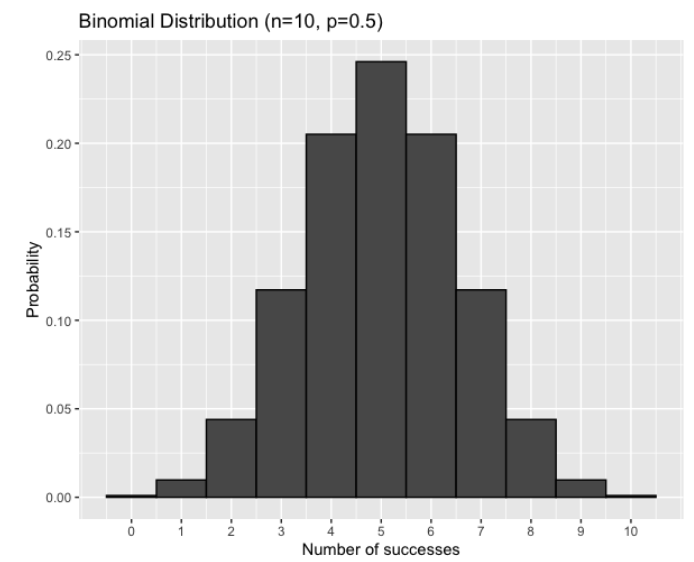
\includegraphics{fig43.png}

\hypertarget{cuuxe1l-es-la-probabilidad-de-7-caras}{%
\subsection{¿Cuál es la probabilidad de 7
caras?}\label{cuuxe1l-es-la-probabilidad-de-7-caras}}

\[
P(caras = 7)?
\]

Para obtener la probabilidad de obtener 7 caras de 10 monedas, podemos
usar \texttt{dbinom()}.

\begin{itemize}
\item
  El primer argumento es el número de caras o éxitos.
\item
  El segundo argumento es el número de intentos, n, y
\item
  El tercer agumento es la probabilidad de éxito p
\end{itemize}

Si lanzamos 10 monedas, hay un 12\% de probabilidad de que 7 de ellas
sean cara.

\begin{Shaded}
\begin{Highlighting}[]
\FunctionTok{dbinom}\NormalTok{(}\DecValTok{7}\NormalTok{, }\DecValTok{10}\NormalTok{, }\FloatTok{0.5}\NormalTok{)}
\end{Highlighting}
\end{Shaded}

\begin{verbatim}
[1] 0.1171875
\end{verbatim}

\hypertarget{cuuxe1l-es-la-probabilidad-de-obtener-muxe1s-de-7-caras}{%
\subsection{¿Cuál es la probabilidad de obtener más de 7
caras?}\label{cuuxe1l-es-la-probabilidad-de-obtener-muxe1s-de-7-caras}}

\[
P(cara > 7)?
\]

Podemos usar el argumento de cola de punto inferior para obtener la
probabilidad de un número de éxitos mayor que el primer argumento. Tenga
en cuenta que esto es lo mismo que 1 menos la misma llamada
\texttt{pbinom}

\begin{Shaded}
\begin{Highlighting}[]
\FunctionTok{pbinom}\NormalTok{(}\DecValTok{7}\NormalTok{, }\DecValTok{10}\NormalTok{, }\FloatTok{0.5}\NormalTok{, }\AttributeTok{lower.tail =} \ConstantTok{FALSE}\NormalTok{)}
\end{Highlighting}
\end{Shaded}

\begin{verbatim}
[1] 0.0546875
\end{verbatim}

\hypertarget{valor-esperado-1}{%
\subsection{Valor Esperado}\label{valor-esperado-1}}

El valor esperado de la distribución binomial se puede calcular
multiplicando \texttt{n} por el \texttt{p}.

\[
\bar{x}= n\times p
\]

El número esperado de caras que obtendremos al lanzar 10 monedas es 10
veces 0.5 que es 5.

\[
\bar{x} = 10\times 0.5 = \fbox{5}
\]

\hypertarget{independencia}{%
\subsection{Independencia}\label{independencia}}

Es importante recordar que para que se aplique la distribución binomial,
cada ensayo debe ser independiente, por lo que el resultado de un ensayo
no debería afectar al siguiente. Por ejemplo, si elegimos al azar de
estas tarjetas con ceros y unos

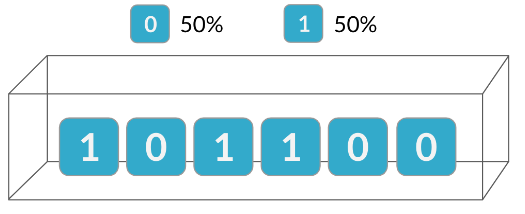
\includegraphics{fig44.png}

Tenemos una probabilidad de 50 - 50 de obtener un 0 un 1.

Pero como estamos muestreando sin reemplazo, las probabilidades para la
segunda prueba son diferentes debido al resultado de la primera prueba.

\includegraphics{fig45.png}

Dado que estos ensayos no son independientes, no podemos calcular
probabilidades precisas para esta situación utilizando la distribución
binomial.

\hypertarget{ejercicio-11}{%
\subsection{Ejercicio 11}\label{ejercicio-11}}

Suponga que Amir generalmente trabaja en 3 tratos por semana y, en
general, gana eñ 30\% de los tratos en los que trabaja. Cada trato tiene
un resultado binario: se \emph{pierde} o se \emph{gana}, por lo que
puede modelar sus tratos de ventas con una distribución binomial. En
este ejercicio, ayudará a Amir a simular un año de sus transacciones
para que pueda comprender mejor su desempeño.

\begin{itemize}
\item
  Primero, establezca una semilla aleatoria en 10 y simule un solo
  trato.

\begin{Shaded}
\begin{Highlighting}[]
\FunctionTok{set.seed}\NormalTok{(}\DecValTok{10}\NormalTok{)}
\FunctionTok{rbinom}\NormalTok{(}\DecValTok{1}\NormalTok{, }\DecValTok{1}\NormalTok{, }\FloatTok{0.3}\NormalTok{)}
\end{Highlighting}
\end{Shaded}

\begin{verbatim}
[1] 0
\end{verbatim}
\item
  Ahora, simule una semana típica de ofertas de Amir, o una semana de 3
  ofertas.

\begin{Shaded}
\begin{Highlighting}[]
\FunctionTok{rbinom}\NormalTok{(}\DecValTok{1}\NormalTok{, }\DecValTok{3}\NormalTok{, }\FloatTok{0.3}\NormalTok{)}
\end{Highlighting}
\end{Shaded}

\begin{verbatim}
[1] 0
\end{verbatim}
\item
  Por último, simule un año de ofertas de Amir, o 52 semanas de 3
  ofertas cada una, y guárdelas en formato \texttt{deals}. Calcule el
  número medio de tratos que ganó por semana.

\begin{Shaded}
\begin{Highlighting}[]
\NormalTok{deals }\OtherTok{\textless{}{-}} \FunctionTok{rbinom}\NormalTok{(}\DecValTok{52}\NormalTok{, }\DecValTok{3}\NormalTok{, }\FloatTok{0.3}\NormalTok{)}

\FunctionTok{mean}\NormalTok{(deals)}
\end{Highlighting}
\end{Shaded}

\begin{verbatim}
[1] 0.8076923
\end{verbatim}
\end{itemize}

\hypertarget{ejercicio-12}{%
\subsection{Ejercicio 12}\label{ejercicio-12}}

Al igual que en el último ejercicio, suponga que A,mir gana el 30\% de
los tratos. Quiere tener una idea de la probabilidad de que cierre una
cierta cantidad de tratos cada semana. En este ejercicio, calculará
cuáles son las probabilidades de que cierre diferentes números de tratos
utilizando la distribución binomial.

\begin{itemize}
\item
  Primero, cuál es la probabilidad de que Amir cierre los 3 tratos en
  una semana?

\begin{Shaded}
\begin{Highlighting}[]
\CommentTok{\# Aquí utilizamos la función de dbinom() puesto que queremos sacar una sola probabilidad de masa, es decir 3 tratos en una semana }
\FunctionTok{dbinom}\NormalTok{(}\DecValTok{3}\NormalTok{, }\DecValTok{3}\NormalTok{, }\FloatTok{0.3}\NormalTok{)}
\end{Highlighting}
\end{Shaded}

\begin{verbatim}
[1] 0.027
\end{verbatim}

  Esto nos dice que de 3 ensayos que hacemos queremos ver las
  probabilidad de que esto ocurra el 100\% de las veces, es decir, 3,
  teniendo en cuenta que la probabilidad de exito es del 30\%.
\item
  ¿cuál es la probabilidad de que Amir cierre 1 trato o menos en una
  semana?

\begin{Shaded}
\begin{Highlighting}[]
\CommentTok{\# }
\CommentTok{\# sin embargo, en este caso, queremos sacar más probabilidades que en el caso anterior, es decir, antes solamente calculabamos la probabilidad de saldar 3 tratos en 1 semana, es decir una solo caso. }
\FunctionTok{pbinom}\NormalTok{(}\DecValTok{1}\NormalTok{, }\DecValTok{3}\NormalTok{, }\FloatTok{0.3}\NormalTok{)}
\end{Highlighting}
\end{Shaded}

\begin{verbatim}
[1] 0.784
\end{verbatim}

  Dicho de otra manera, queremos saber cual es la probabilidad de que el
  éxito, ocurra una vez en 3, teniendo en cuenta que la probabilidad es
  del 30\%.
\item
  ¿Cuál es la probabilidad de que Amir cierre más de 1 trato?

\begin{Shaded}
\begin{Highlighting}[]
\FunctionTok{pbinom}\NormalTok{(}\DecValTok{1}\NormalTok{, }\DecValTok{3}\NormalTok{, }\FloatTok{0.3}\NormalTok{, }\AttributeTok{lower.tail =} \ConstantTok{FALSE}\NormalTok{)}
\end{Highlighting}
\end{Shaded}

\begin{verbatim}
[1] 0.216
\end{verbatim}

  Lo que estamos viendo en este caso, es ver cual es la probabilidad de
  tener por lo menos, 1 éxito, o más 2 o incluso 3, de tres ensayos.
\end{itemize}

\hypertarget{ejercicio-13}{%
\subsection{Ejercicio 13}\label{ejercicio-13}}

Ahora amir quiere saber cuántos tratos puede esperar cerrar cada semana
si cambia su tasa de ganancias. Afortunadamente, puede usar su
conocimiento de distribución binomial para ayudarlo a calcular el valor
esperado en diferentes situaciones.

\begin{itemize}
\item
  Primero, calcule el número esperado de ventas de las 3 en las que
  trabaja que Amir ganará cada semana si mantiene su tasa de ganancia
  del 30\%.

\begin{Shaded}
\begin{Highlighting}[]
\NormalTok{won\_30pct }\OtherTok{\textless{}{-}} \DecValTok{3} \SpecialCharTok{*} \FloatTok{0.3}
\NormalTok{won\_30pct}
\end{Highlighting}
\end{Shaded}

\begin{verbatim}
[1] 0.9
\end{verbatim}
\item
  Segundo, calcule el número esperado de ventas de las 3 en las que
  trabaja que ganará si su tasa de ganancias cae al 25\%.

\begin{Shaded}
\begin{Highlighting}[]
\NormalTok{won\_25pct }\OtherTok{\textless{}{-}} \DecValTok{3} \SpecialCharTok{*}\FloatTok{0.25}
\NormalTok{won\_25pct}
\end{Highlighting}
\end{Shaded}

\begin{verbatim}
[1] 0.75
\end{verbatim}
\item
  Tercero, calcule la cantidad esperada de ventas de las 3 en las que
  trabaja que ganará si su tasa de ganancias aumenta al 35\%.

\begin{Shaded}
\begin{Highlighting}[]
\NormalTok{won\_35pct }\OtherTok{\textless{}{-}} \DecValTok{3} \SpecialCharTok{*} \FloatTok{0.35}
\NormalTok{won\_35pct}
\end{Highlighting}
\end{Shaded}

\begin{verbatim}
[1] 1.05
\end{verbatim}
\end{itemize}

\bookmarksetup{startatroot}

\hypertarget{references}{%
\chapter*{References}\label{references}}
\addcontentsline{toc}{chapter}{References}

\markboth{References}{References}

\hypertarget{refs}{}
\begin{CSLReferences}{0}{0}
\end{CSLReferences}



\end{document}
